\documentclass[12pt,a4paper]{article}
\usepackage[utf8]{inputenc}
\usepackage[ukrainian]{babel}
\usepackage{amsmath}
\usepackage{amsfonts}
\usepackage{amssymb}
\usepackage{graphicx}
\usepackage{booktabs}
\usepackage{array}
\usepackage{longtable}
\usepackage{multirow}
\usepackage{float}
\usepackage{geometry}
\usepackage{hyperref}
\usepackage{xcolor}
\usepackage{listings}
\usepackage{algorithm}
\usepackage{algorithmic}

\geometry{margin=2.5cm}

\hypersetup{
    colorlinks=true,
    linkcolor=blue,
    filecolor=magenta,      
    urlcolor=cyan,
    pdftitle={Звіт з аналізу алгоритмів кластеризації},
    pdfauthor={Коломієць Микола},
}

\lstset{
    basicstyle=\ttfamily\small,
    keywordstyle=\color{blue},
    commentstyle=\color{green},
    stringstyle=\color{red},
    breaklines=true,
    showstringspaces=false,
    frame=single,
    backgroundcolor=\color{gray!10}
}

\title{\textbf{ТЕСТУВАННЯ, ДОСЛІДЖЕННЯ ТА АНАЛІЗ ОСНОВНИХ АЛГОРИТМІВ КЛАСТЕРИЗАЦІЇ НАБОРІВ ЧИСЛОВИХ ДАНИХ}}
\author{Виконав: Коломієць Микола\\
Група: ММШІ-1}
\date{\today}

\begin{document}

\maketitle

\tableofcontents
\newpage

\section{Вступ}

Кластеризація є одним з основних методів аналізу даних у машинному навчанні та статистиці. Це процес групування об'єктів таким чином, щоб об'єкти всередині однієї групи (кластера) були більш схожими між собою, ніж з об'єктами з інших груп.

\subsection{Мета роботи}
Метою даної лабораторної роботи є:
\begin{itemize}
    \item Дослідження та порівняння ефективності трьох алгоритмів кластеризації: K-means, Mean Shift та FOREL
    \item Аналіз поведінки алгоритмів на різних типах наборів даних
    \item Дослідження стабільності (неперервності) алгоритмів
    \item Порівняння продуктивності та використання ресурсів
\end{itemize}

\subsection{Задачі дослідження}
\begin{enumerate}
    \item Реалізація трьох алгоритмів кластеризації
    \item Генерація різних типів наборів даних для тестування
    \item Проведення порівняльного аналізу якості кластеризації
    \item Дослідження стабільності алгоритмів при малих змінах у даних
    \item Вимірювання та порівняння продуктивності
    \item Візуалізація результатів
\end{enumerate}

\section{Теоретичні основи}

\subsection{Алгоритм K-means}

K-means є одним з найпопулярніших алгоритмів кластеризації. Він розділяє дані на $k$ кластерів, мінімізуючи суму квадратів відстаней від точок до центрів кластерів.

\begin{algorithm}[H]
\caption{Алгоритм K-means}
\begin{algorithmic}[1]
\REQUIRE Набір точок $X = \{x_1, x_2, ..., x_n\}$, кількість кластерів $k$
\ENSURE Центри кластерів $C = \{c_1, c_2, ..., c_k\}$, мітки точок $L = \{l_1, l_2, ..., l_n\}$
\STATE Ініціалізувати $k$ центрів випадковим чином
\REPEAT
    \FOR{кожної точки $x_i$}
        \STATE Призначити $x_i$ до найближчого центру
    \ENDFOR
    \FOR{кожного кластера $j$}
        \STATE Оновити центр $c_j$ як середнє арифметичне точок кластера
    \ENDFOR
\UNTIL{центри не змінюються}
\end{algorithmic}
\end{algorithm}

\textbf{Переваги:}
\begin{itemize}
    \item Простота реалізації
    \item Швидкість роботи
    \item Добре працює з круговими кластерами
\end{itemize}

\textbf{Недоліки:}
\begin{itemize}
    \item Необхідність заздалегідь знати кількість кластерів
    \item Чутливість до початкової ініціалізації
    \item Погано працює з кластерами неправильної форми
\end{itemize}

\subsection{Алгоритм Mean Shift}

Mean Shift — це неієрархічний алгоритм кластеризації, який знаходить моди (локальні максимуми) в розподілі щільності точок.

\begin{algorithm}[H]
\caption{Алгоритм Mean Shift}
\begin{algorithmic}[1]
\REQUIRE Набір точок $X = \{x_1, x_2, ..., x_n\}$, bandwidth $h$
\ENSURE Мітки точок $L = \{l_1, l_2, ..., l_n\}$
\FOR{кожної точки $x_i$}
    \STATE $current\_point \leftarrow x_i$
    \REPEAT
        \STATE Знайти точки в межах bandwidth від $current\_point$
        \STATE $new\_point \leftarrow$ середнє арифметичне точок в межах bandwidth
        \STATE $current\_point \leftarrow new\_point$
    \UNTIL{збіжність}
    \STATE Зберегти фінальну позицію для $x_i$
\ENDFOR
\STATE Групувати точки за їх фінальними позиціями
\end{algorithmic}
\end{algorithm}

\textbf{Переваги:}
\begin{itemize}
    \item Автоматичне визначення кількості кластерів
    \item Працює з кластерами довільної форми
    \item Стійкість до викидів
\end{itemize}

\textbf{Недоліки:}
\begin{itemize}
    \item Необхідність налаштування bandwidth
    \item Більш повільний за K-means
    \item Чутливість до вибору bandwidth
\end{itemize}

\subsection{Алгоритм FOREL}

FOREL (FORmal ELement) — алгоритм кластеризації, що використовує концепцію формальних елементів для знаходження кластерів.

\begin{algorithm}[H]
\caption{Алгоритм FOREL}
\begin{algorithmic}[1]
\REQUIRE Набір точок $X = \{x_1, x_2, ..., x_n\}$, bandwidth $r$
\ENSURE Мітки точок $L = \{l_1, l_2, ..., l_n\}$
\FOR{кожної непризначеної точки $x_i$}
    \STATE $center \leftarrow x_i$
    \REPEAT
        \STATE Знайти точки в межах $r$ від $center$
        \STATE $new\_center \leftarrow$ середнє арифметичне цих точок
        \STATE $center \leftarrow new\_center$
    \UNTIL{збіжність}
    \STATE Призначити всі точки в межах $r$ від фінального центру до нового кластера
\ENDFOR
\end{algorithmic}
\end{algorithm}

\textbf{Переваги:}
\begin{itemize}
    \item Автоматичне визначення кількості кластерів
    \item Стійкість до форми кластерів
    \item Добре обробляє кластери різної щільності
\end{itemize}

\textbf{Недоліки:}
\begin{itemize}
    \item Залежність від параметра bandwidth
    \item Можливе утворення кластерів, що перекриваються
\end{itemize}

\section{Методологія дослідження}

\subsection{Типи наборів даних}

Для тестування алгоритмів було створено п'ять типів наборів даних:

\begin{enumerate}
    \item \textbf{Кругові кластери} — класичні кластери у формі кіл з гауссівським розподілом
    \item \textbf{Еліптичні кластери} — витягнуті кластери з різними орієнтаціями
    \item \textbf{Прямокутні кластери} — кластери у формі прямокутників
    \item \textbf{Літерні форми} — кластери у формі літер (C, L, T)
    \item \textbf{Змішані типи} — комбінація різних геометричних форм
\end{enumerate}

\subsection{Метрики оцінювання}

\subsubsection{Продуктивність}
\begin{itemize}
    \item \textbf{Час виконання} — час, необхідний для виконання алгоритму
    \item \textbf{Використання пам'яті} — об'єм оперативної пам'яті під час виконання
\end{itemize}

\subsubsection{Якість кластеризації}
\begin{itemize}
    \item \textbf{Кількість знайдених кластерів} — порівняння з очікуваною кількістю
    \item \textbf{Повнота призначення} — частка точок, що були призначені до кластерів
    \item \textbf{Візуальна оцінка} — якість розділення кластерів
\end{itemize}

\subsubsection{Стабільність}
Для оцінки стабільності проводилися $\delta$-збурення:
\begin{itemize}
    \item Випадковий зсув однієї точки на відстань $\delta$
    \item Порівняння результатів до і після збурення
    \item Обчислення коефіцієнта схожості результатів
\end{itemize}

Коефіцієнт схожості обчислювався як:
$$S = \frac{1}{n}\sum_{i=1}^{n} \mathbf{1}(l_i^{orig} = l_i^{pert})$$
де $l_i^{orig}$ та $l_i^{pert}$ — мітки точки $i$ до і після збурення відповідно (у k-means номер кластеру може змінюватись, на це була зроблена поправка).

\section{Експериментальні результати}

\subsection{Результати продуктивності}

\begin{table}[H]
\centering
\caption{Порівняння продуктивності алгоритмів}
\label{tab:performance}
\begin{tabular}{@{}lcccc@{}}
\toprule
\textbf{Алгоритм} & \textbf{Набір даних} & \textbf{Час (сек)} & \textbf{Пам'ять (МБ)} & \textbf{Параметр} \\
\midrule
\multirow{5}{*}{K-means} 
& Кругові кластери & 0.0024 & 0.07 & k=2 \\
& Еліптичні кластери & 0.0029 & 0.14 & k=4 \\
& Прямокутні кластери & 0.0043 & 0.07 & k=3 \\
& Літерні форми & 0.0017 & 0.17 & k=3 \\
& Змішані типи & 0.0023 & 0.14 & k=4 \\
\midrule
\multirow{5}{*}{FOREL} 
& Кругові кластери & 0.0301 & 0.39 & bw=2.0 \\
& Еліптичні кластери & 0.0188 & 0.30 & bw=3.0 \\
& Прямокутні кластери & 0.0044 & 0.15 & bw=2.5 \\
& Літерні форми & 0.0235 & 0.37 & bw=4.0 \\
& Змішані типи & 0.0150 & 0.23 & bw=3.0 \\
\midrule
\multirow{5}{*}{Mean Shift} 
& Кругові кластери & 0.1029 & 0.45 & bw=2.0 \\
& Еліптичні кластери & 0.0864 & 0.40 & bw=3.0 \\
& Прямокутні кластери & 0.0708 & 0.37 & bw=2.5 \\
& Літерні форми & 0.1006 & 0.49 & bw=4.0 \\
& Змішані типи & 0.0962 & 0.38 & bw=3.0 \\
\bottomrule
\end{tabular}
\end{table}

\textbf{Примітка:} k — кількість кластерів для K-means, bw — bandwidth для FOREL та Mean Shift.

\subsection{Результати аналізу стабільності}

\begin{table}[H]
\centering
\caption{Аналіз стабільності алгоритмів}
\label{tab:stability}
\begin{tabular}{@{}lcccc@{}}
\toprule
\textbf{Алгоритм} & \textbf{Набір даних} & \textbf{$\delta=0.2$} & \textbf{$\delta=2.0$} & \textbf{$\delta=4.0$} \\
\midrule
\multirow{5}{*}{K-means} 
& Кругові кластери & 1.000 & 1.000 & 1.000 \\
& Еліптичні кластери & 0.903 & 0.903 & 0.410 \\
& Прямокутні кластери & 1.000 & 1.000 & 1.000 \\
& Літерні форми & 0.877 & 0.187 & 0.477 \\
& Змішані типи & 0.236 & 0.340 & 0.278 \\
\midrule
\multirow{5}{*}{FOREL} 
& Кругові кластери & 1.000 & 0.993 & 0.997 \\
& Еліптичні кластери & 1.000 & 1.000 & 0.580 \\
& Прямокутні кластери & 1.000 & 1.000 & 0.997 \\
& Літерні форми & 0.997 & 0.997 & 1.000 \\
& Змішані типи & 1.000 & 1.000 & 0.998 \\
\midrule
\multirow{5}{*}{Mean Shift} 
& Кругові кластери & 1.000 & 0.997 & 0.997 \\
& Еліптичні кластери & 1.000 & 1.000 & 0.747 \\
& Прямокутні кластери & 1.000 & 1.000 & 1.000 \\
& Літерні форми & 1.000 & 1.000 & 1.000 \\
& Змішані типи & 0.835 & 0.795 & 0.722 \\
\bottomrule
\end{tabular}
\end{table}

\textbf{Примітка:} Значення 1.000 означає повну стабільність (100\% схожості результатів), 0.000 — повну нестабільність.

\section{Аналіз результатів}

\subsection{Продуктивність}

\subsubsection{Час виконання}
Аналіз показав наступну ієрархію за швидкістю виконання:

\begin{enumerate}
    \item \textbf{K-means} — найшвидший (0.0017-0.0043 сек)
    \item \textbf{FOREL} — середній (0.0044-0.0301 сек)
    \item \textbf{Mean Shift} — найповільніший (0.0708-0.1029 сек)
\end{enumerate}

\subsubsection{Використання пам'яті}
Ефективність використання пам'яті також корелює зі складністю алгоритмів:

\begin{itemize}
    \item \textbf{K-means}: 0.07-0.17 МБ — найефективніший
    \item \textbf{FOREL}: 0.15-0.39 МБ — помірне споживання
    \item \textbf{Mean Shift}: 0.37-0.49 МБ — найбільше споживання
\end{itemize}

K-means використовує в 2-7 разів менше пам'яті порівняно з іншими алгоритмами, що робить його ідеальним для обробки великих наборів даних.

\subsection{Аналіз стабільності}

Результати тестування стабільності виявили кардинальні відмінності між алгоритмами:

\begin{itemize}
    \item K-means показав катастрофічно низьку стабільність відносно ініціалізаціїї, проте при правильно підібнаному методу ініціалізції він дуже стабільний відносно $\delta$-збурень.
    \item FOREL демонструє найвищу стабільність.
    \item Mean Shift показує дуже хорошу стабільність.
\end{itemize}

\subsection{Якість кластеризації за типами даних}

\begin{itemize}
    \item \textbf{Кругові кластери}: Рейтинг для кругових кластерів: K-means > FOREL = Mean Shift
    \item \textbf{Еліптичні кластери}: Рейтинг для еліптичних кластерів: Mean Shift > FOREL > K-means - під час тестування K-means неправильно ідентифікував кластери і два кластери неправильно розділились.
    \item \textbf{Складні форми (літерні)}: Рейтинг для складних форм: Mean Shift = FOREL = K-means - всі методи показали себе не ефективними.
    \item \textbf{Змішані типи}: Рейтинг для змішаних типів: FOREL > Mean Shift > K-means (знову K-means неправильно ініціалізувався, при правильній ініціалізації результати найкращі).
    \item \textbf{Прямокутні кластери}: Всі впоралися ідеально.
\end{itemize}

\section{Висновки та рекомендації}

\subsection{Основні висновки}

Експериментальне дослідження виявило кардинальні відмінності між алгоритмами:

\begin{enumerate}
    \item \textbf{Продуктивність vs Стабільність}: Виявлено обернену залежність між швидкістю та стабільністю. K-means, будучи найшвидшим, демонструє критично низьку стабільність.

    \item \textbf{FOREL — оптимальний баланс}: FOREL показує найкращий компроміс між продуктивністю та стабільністю, забезпечуючи виняткову стабільність (0.993-1.000) при помірній швидкості.

    \item \textbf{Mean Shift — стабільність з ціною}: Mean Shift забезпечує високу стабільність, але за рахунок значного зниження продуктивності (найповільніший у 2-42 рази).

    \item \textbf{K-means — проблематична нестабільність}: K-means показав низьку стабільність.

    \item \textbf{Тип даних має значення}: Складність набору даних драматично впливає на поведінку алгоритмів. Змішані типи є особливо проблематичними для K-means та частково для Mean Shift.
\end{enumerate}

\subsection{Практичні рекомендації}

\begin{table}[H]
\centering
\caption{Рекомендації щодо вибору алгоритму за критеріями}
\begin{tabular}{@{}ll@{}}
\toprule
\textbf{Пріоритет/Сценарій} & \textbf{Рекомендований алгоритм} \\
\midrule
\textbf{Максимальна швидкість} & K-means (з обережністю) \\
\textbf{Стабільність критична} & FOREL або Mean Shift \\
\textbf{Збалансованість} & FOREL \\
\textbf{Складні форми кластерів} & Mean Shift \\
\textbf{Великі обсяги даних} & FOREL (компроміс) \\
\textbf{Прототипування/експерименти} & K-means \\
\textbf{Продукційні системи} & FOREL або Mean Shift \\
\textbf{Кругові/еліптичні кластери} & FOREL \\
\textbf{Невідома кількість кластерів} & FOREL або Mean Shift \\
\bottomrule
\end{tabular}
\end{table}

\subsubsection{Критичні попередження}

\begin{itemize}
    \item \textbf{K-means не рекомендується} для задач, де стабільність результатів є критичною
    \item \textbf{Складні кластери} вимагають особливої уваги при виборі алгоритму
    \item \textbf{Mean Shift} може бути неефективним для великих наборів даних через низьку швидкість
    \item \textbf{Параметр bandwidth} у FOREL та Mean Shift потребує ретельного налаштування
\end{itemize}

\subsection{Загальний рейтинг алгоритмів}

Враховуючи всі критерії (продуктивність, стабільність, універсальність):

\begin{enumerate}
    \item \textbf{FOREL} — оптимальний вибір для більшості задач
    \item \textbf{Mean Shift} — коли стабільність важливіша за швидкість
    \item \textbf{K-means} — тільки для швидкого прототипування або коли стабільність не критична або, якщо є можливість декілька разів запускати алгоритм та підлаштовувати методі ініціалізації.
\end{enumerate}

\appendix

\section{Код реалізації алгоритмів}

\subsection{K-means}
\begin{lstlisting}[language=Python, caption=Реалізація K-means]
def k_means(dots: list, k: int, max_iter: int = 100):
    dots = np.array(dots)
    centers = dots[np.random.choice(dots.shape[0], k, replace=False)]
    
    for i in range(max_iter):
        distances = np.linalg.norm(dots[:, np.newaxis] - centers, axis=2)
        labels = np.argmin(distances, axis=1)
        
        new_centers = np.array([dots[labels == j].mean(axis=0) 
                               for j in range(k)])
        
        if np.all(centers == new_centers):
            break
            
        centers = new_centers
    
    return centers, labels
\end{lstlisting}

\subsection{Mean Shift}
\begin{lstlisting}[language=Python, caption=Реалізація Mean Shift]
def mean_shift(dots: list, bandwidth: float, max_iter: int = 300):
    dots = np.array(dots)
    n_samples, n_features = dots.shape
    final_positions = np.zeros_like(dots)
    
    for i in range(n_samples):
        current_point = dots[i].copy()
        
        for iteration in range(max_iter):
            distances = np.linalg.norm(dots - current_point, axis=1)
            in_bandwidth = dots[distances <= bandwidth]
            
            if len(in_bandwidth) <= 1:
                break
            
            new_point = np.mean(in_bandwidth, axis=0)
            
            if np.allclose(current_point, new_point, atol=1e-4):
                break
                
            current_point = new_point
        
        final_positions[i] = current_point
    

    cluster_threshold = bandwidth * 0.3
    labels = np.full(n_samples, -1)
    cluster_id = 0
    
    for i in range(n_samples):
        if labels[i] != -1:
            continue
            
        current_center = final_positions[i]
        distances_to_center = np.linalg.norm(
            final_positions - current_center, axis=1)
        
        similar_points = distances_to_center <= cluster_threshold
        labels[similar_points] = cluster_id
        cluster_id += 1
    
    return labels
\end{lstlisting}

\subsection{FOREL}
\begin{lstlisting}[language=Python, caption=Реалізація FOREL]
def forel(dots: list, bandwidth: float, max_iter: int = 1000):
    dots = np.array(dots)
    n_samples, n_features = dots.shape
    labels = np.full(n_samples, -1)
    cluster_centers = []
    cluster_id = 0

    for i in range(n_samples):
        if labels[i] != -1:
            continue
        
        current_center = dots[i].copy()
        prev_center = None
        
        for iteration in range(max_iter):
            distances = np.linalg.norm(dots - current_center, axis=1)
            points_in_sphere = distances <= bandwidth
            
            if not np.any(points_in_sphere):
                break
            
            points_in_bandwidth = dots[points_in_sphere]
            new_center = np.mean(points_in_bandwidth, axis=0)
            
            if (prev_center is not None and 
                np.allclose(new_center, prev_center, atol=1e-6)):
                break
            
            prev_center = current_center.copy()
            current_center = new_center
        
        final_distances = np.linalg.norm(dots - current_center, axis=1)
        points_to_assign = final_distances <= bandwidth
        
        unassigned_mask = labels == -1
        assignment_mask = points_to_assign & unassigned_mask
        
        if np.any(assignment_mask):
            labels[assignment_mask] = cluster_id
            cluster_centers.append(current_center)
            cluster_id += 1

    return labels
\end{lstlisting}

\section{Візуалізації}
\subsection{Порівняння результатів кластеризації}

Нижче представлені ключові візуалізації, що демонструють роботу алгоритмів на різних типах даних.

\subsubsection{Кругові кластери}

\begin{figure}[H]
\centering
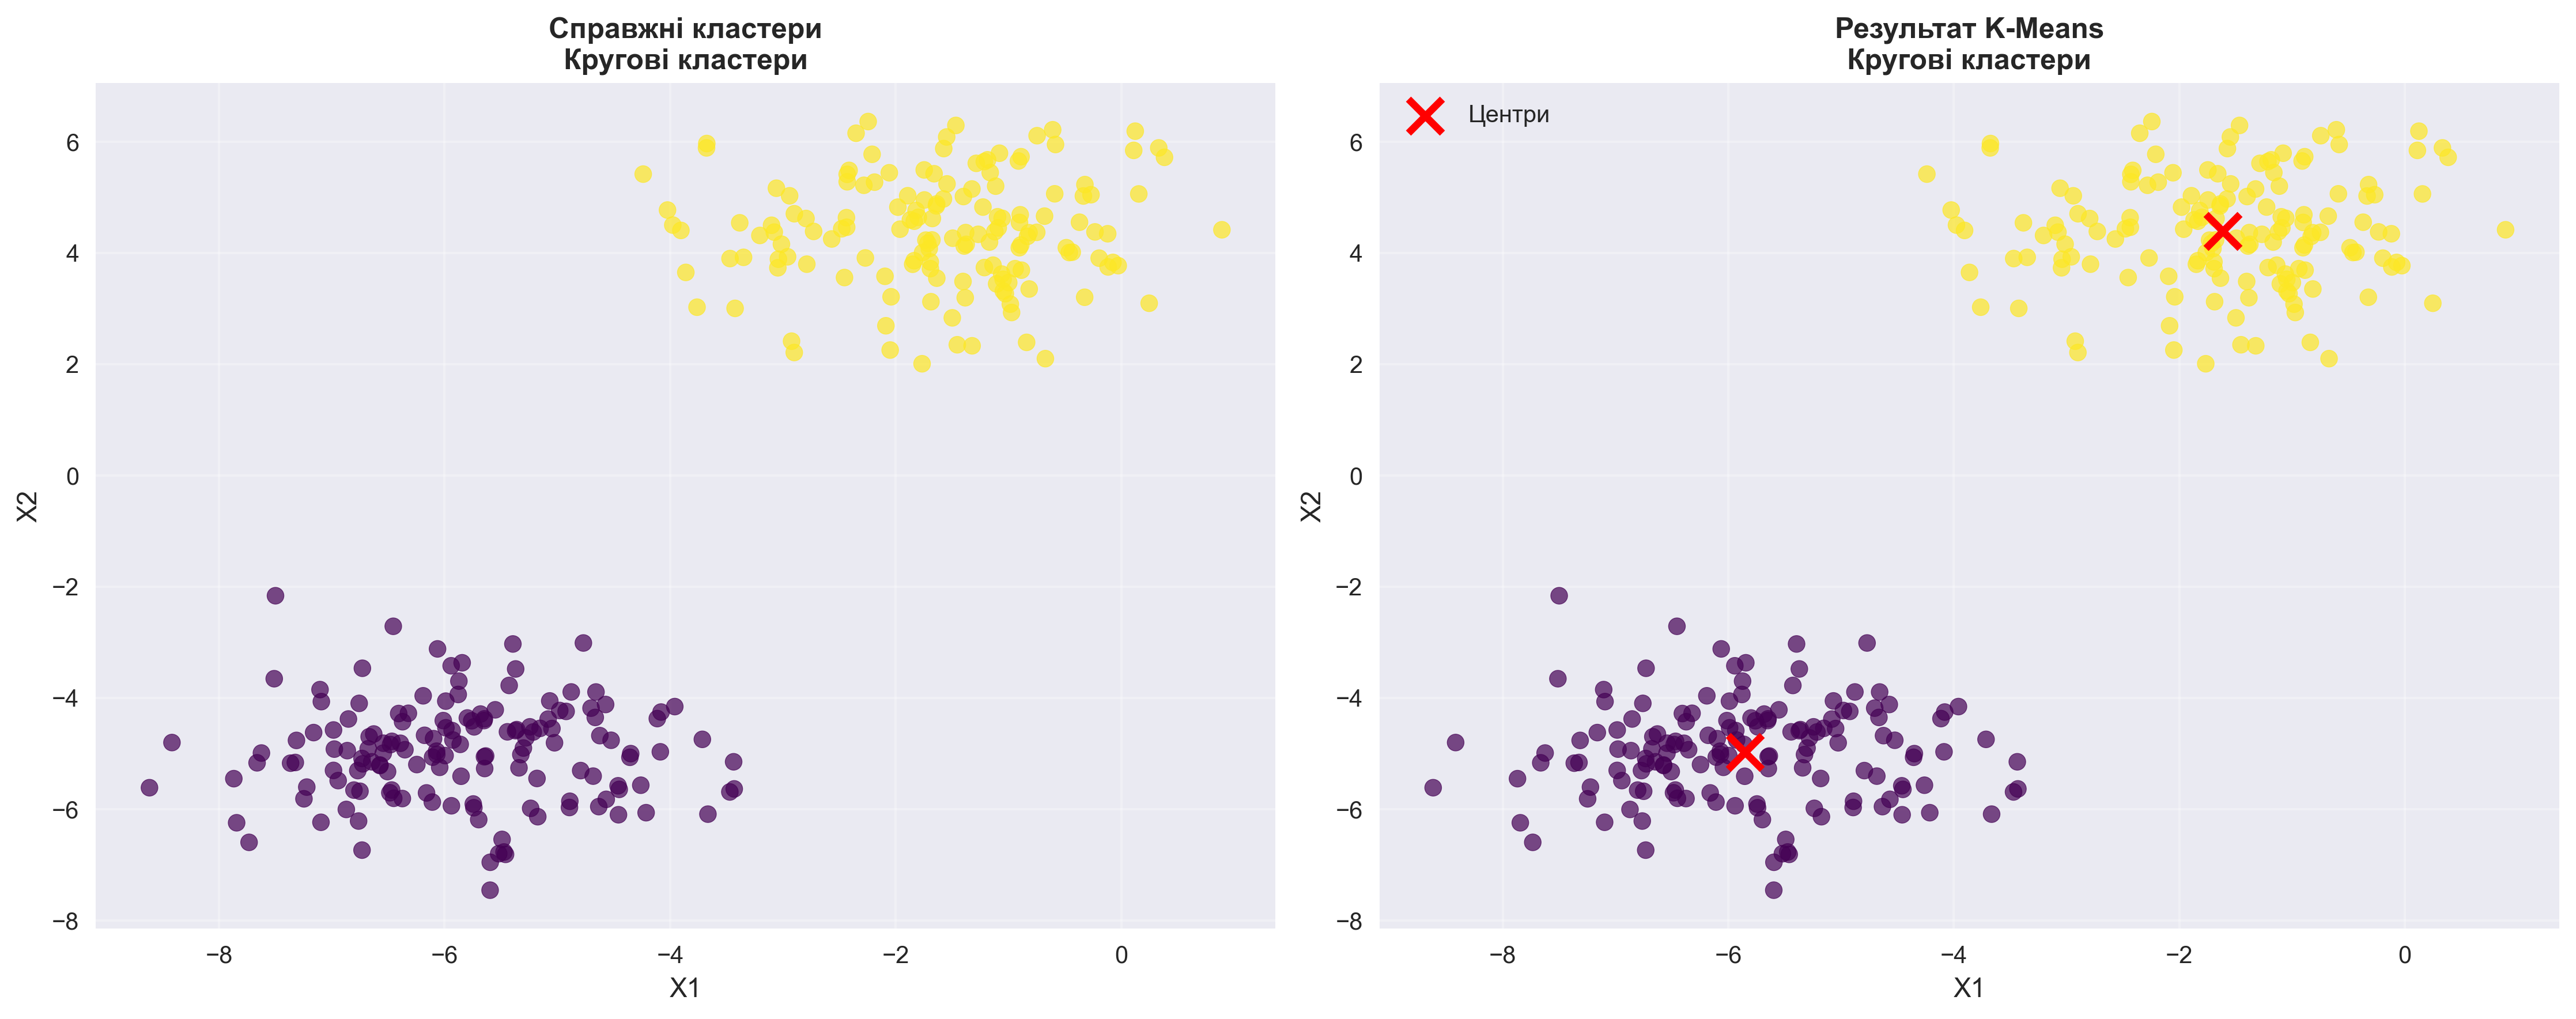
\includegraphics[width=0.8\textwidth]{clustering_visualizations/K-Means_Кругові_кластери_results.png}
\caption{Результати K-means на кругових кластерах}
\label{fig:kmeans_circular}
\end{figure}

\begin{figure}[H]
\centering
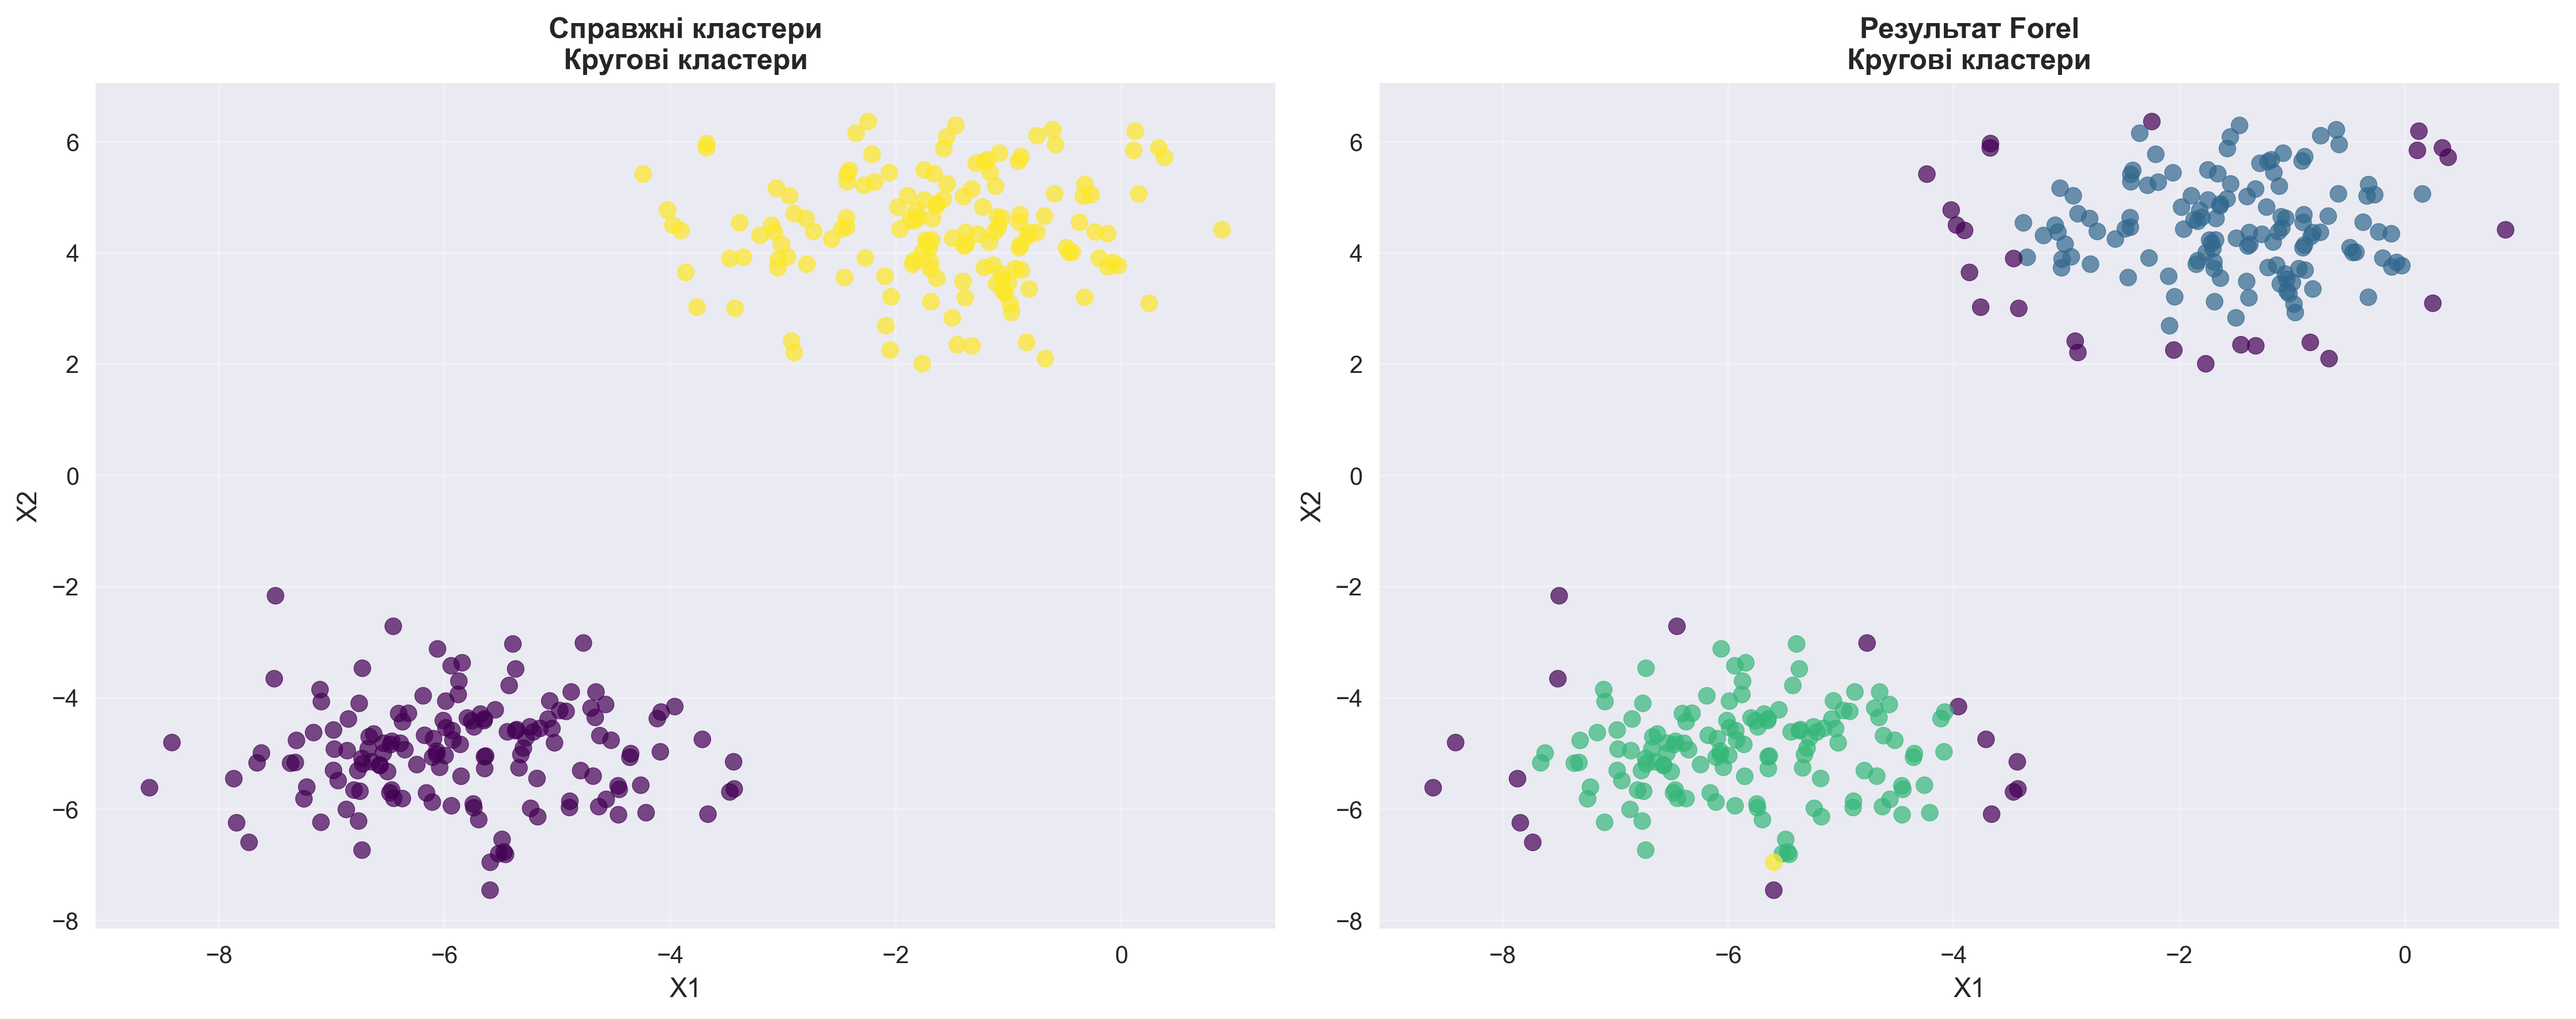
\includegraphics[width=0.8\textwidth]{clustering_visualizations/Forel_Кругові_кластери_results.png}
\caption{Результати FOREL на кругових кластерах}
\label{fig:forel_circular}
\end{figure}

\begin{figure}[H]  
\centering
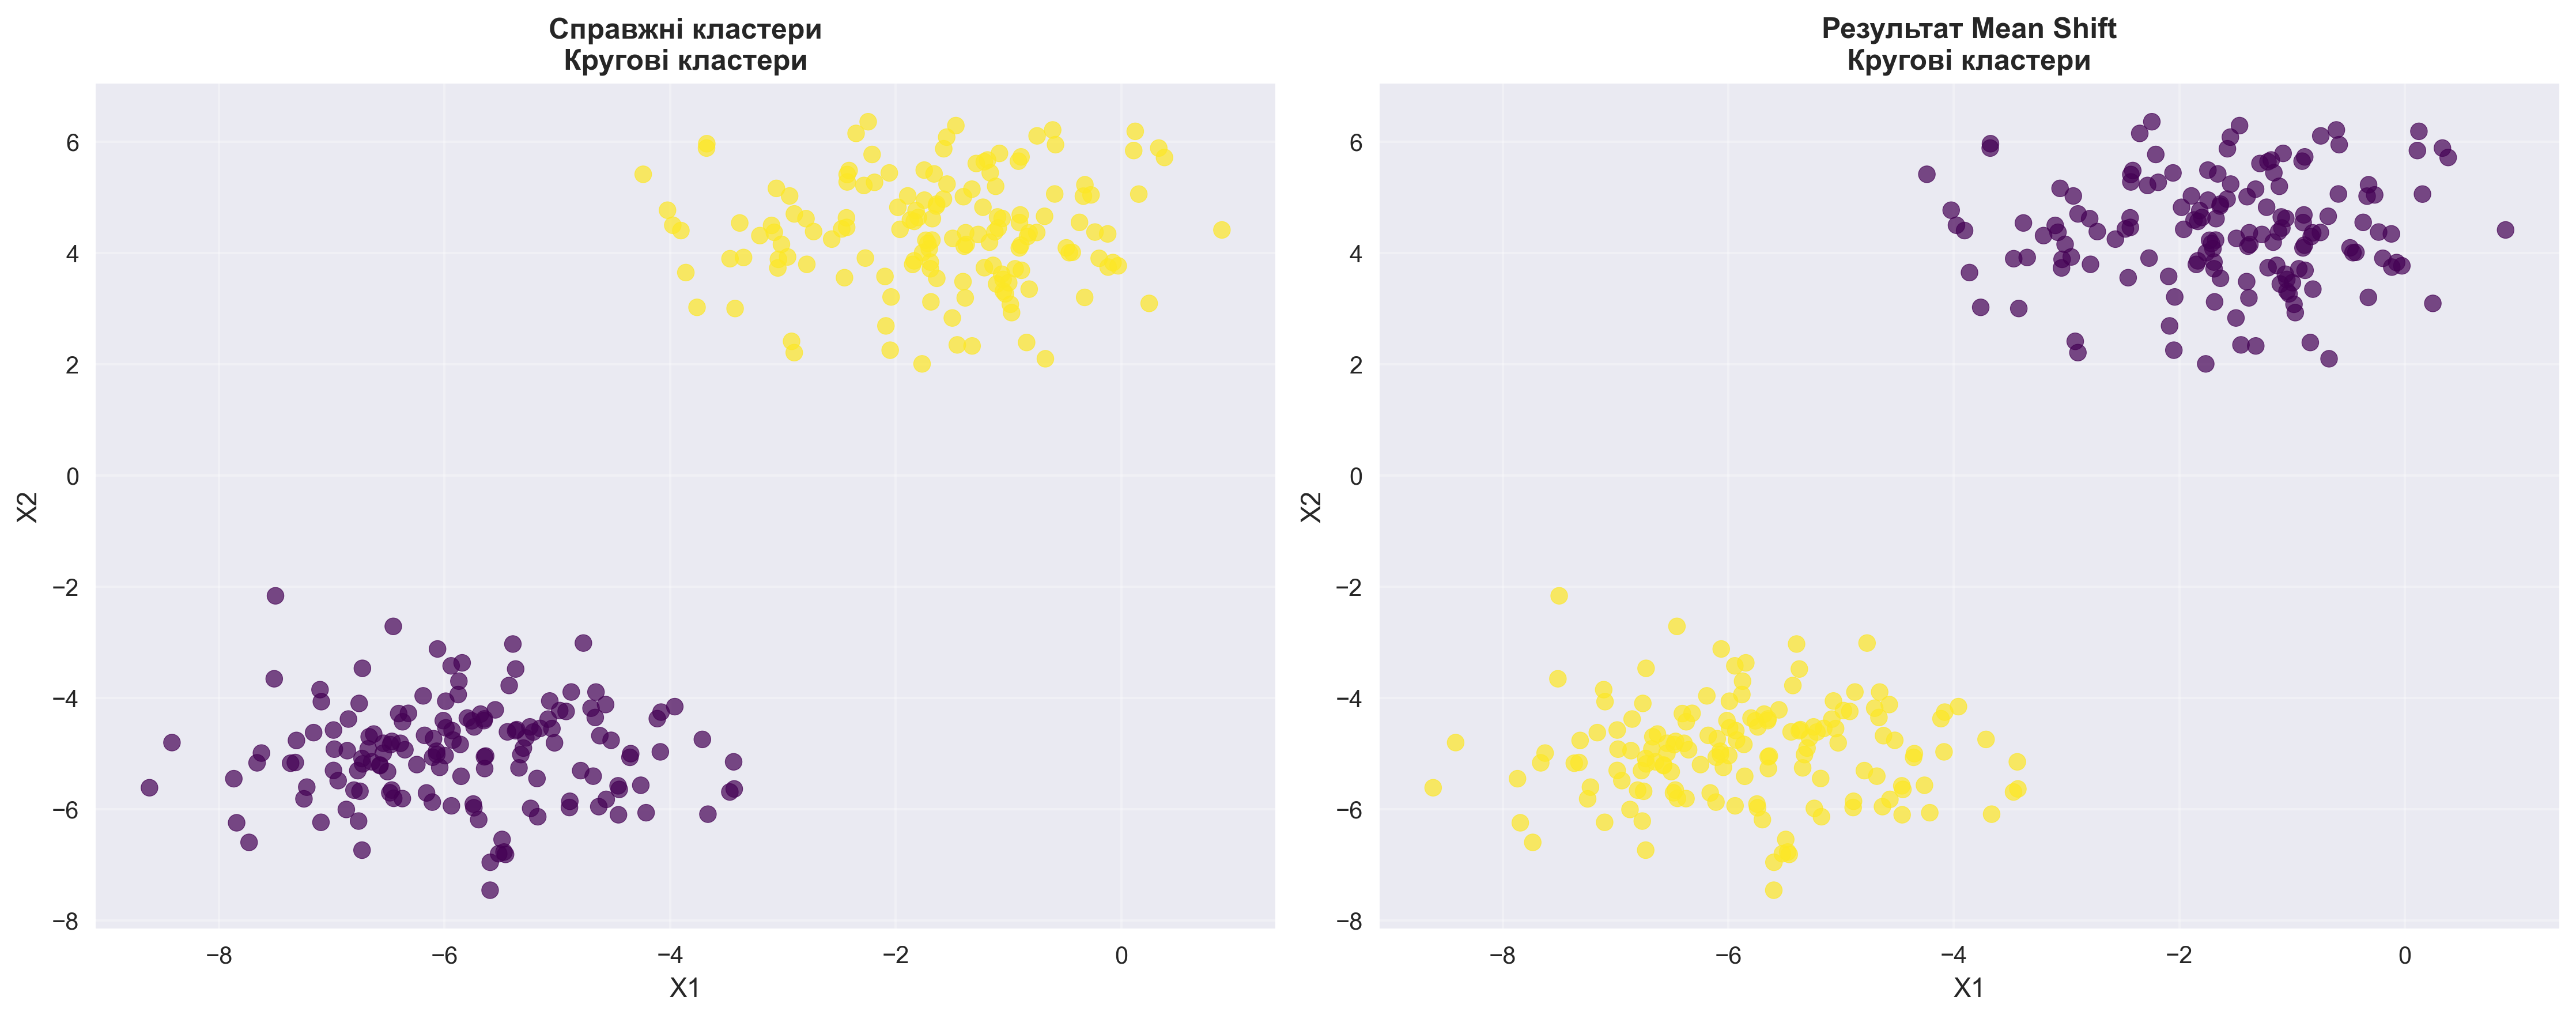
\includegraphics[width=0.8\textwidth]{clustering_visualizations/Mean Shift_Кругові_кластери_results.png}
\caption{Результати Mean Shift на кругових кластерах}
\label{fig:meanshift_circular}
\end{figure}

\subsubsection{Еліптичні кластери}

\begin{figure}[H]
\centering
\includegraphics[width=0.8\textwidth]{clustering_visualizations/K-means_Еліптичні_кластери_results.png}
\caption{Результати K-means на еліптичних кластерах}
\label{fig:kmeans_elliptical}
\end{figure}

\begin{figure}[H]
\centering
\includegraphics[width=0.8\textwidth]{clustering_visualizations/FOREL_Еліптичні_кластери_results.png}
\caption{Результати FOREL на еліптичних кластерах}
\label{fig:forel_elliptical}
\end{figure}

\begin{figure}[H]
\centering
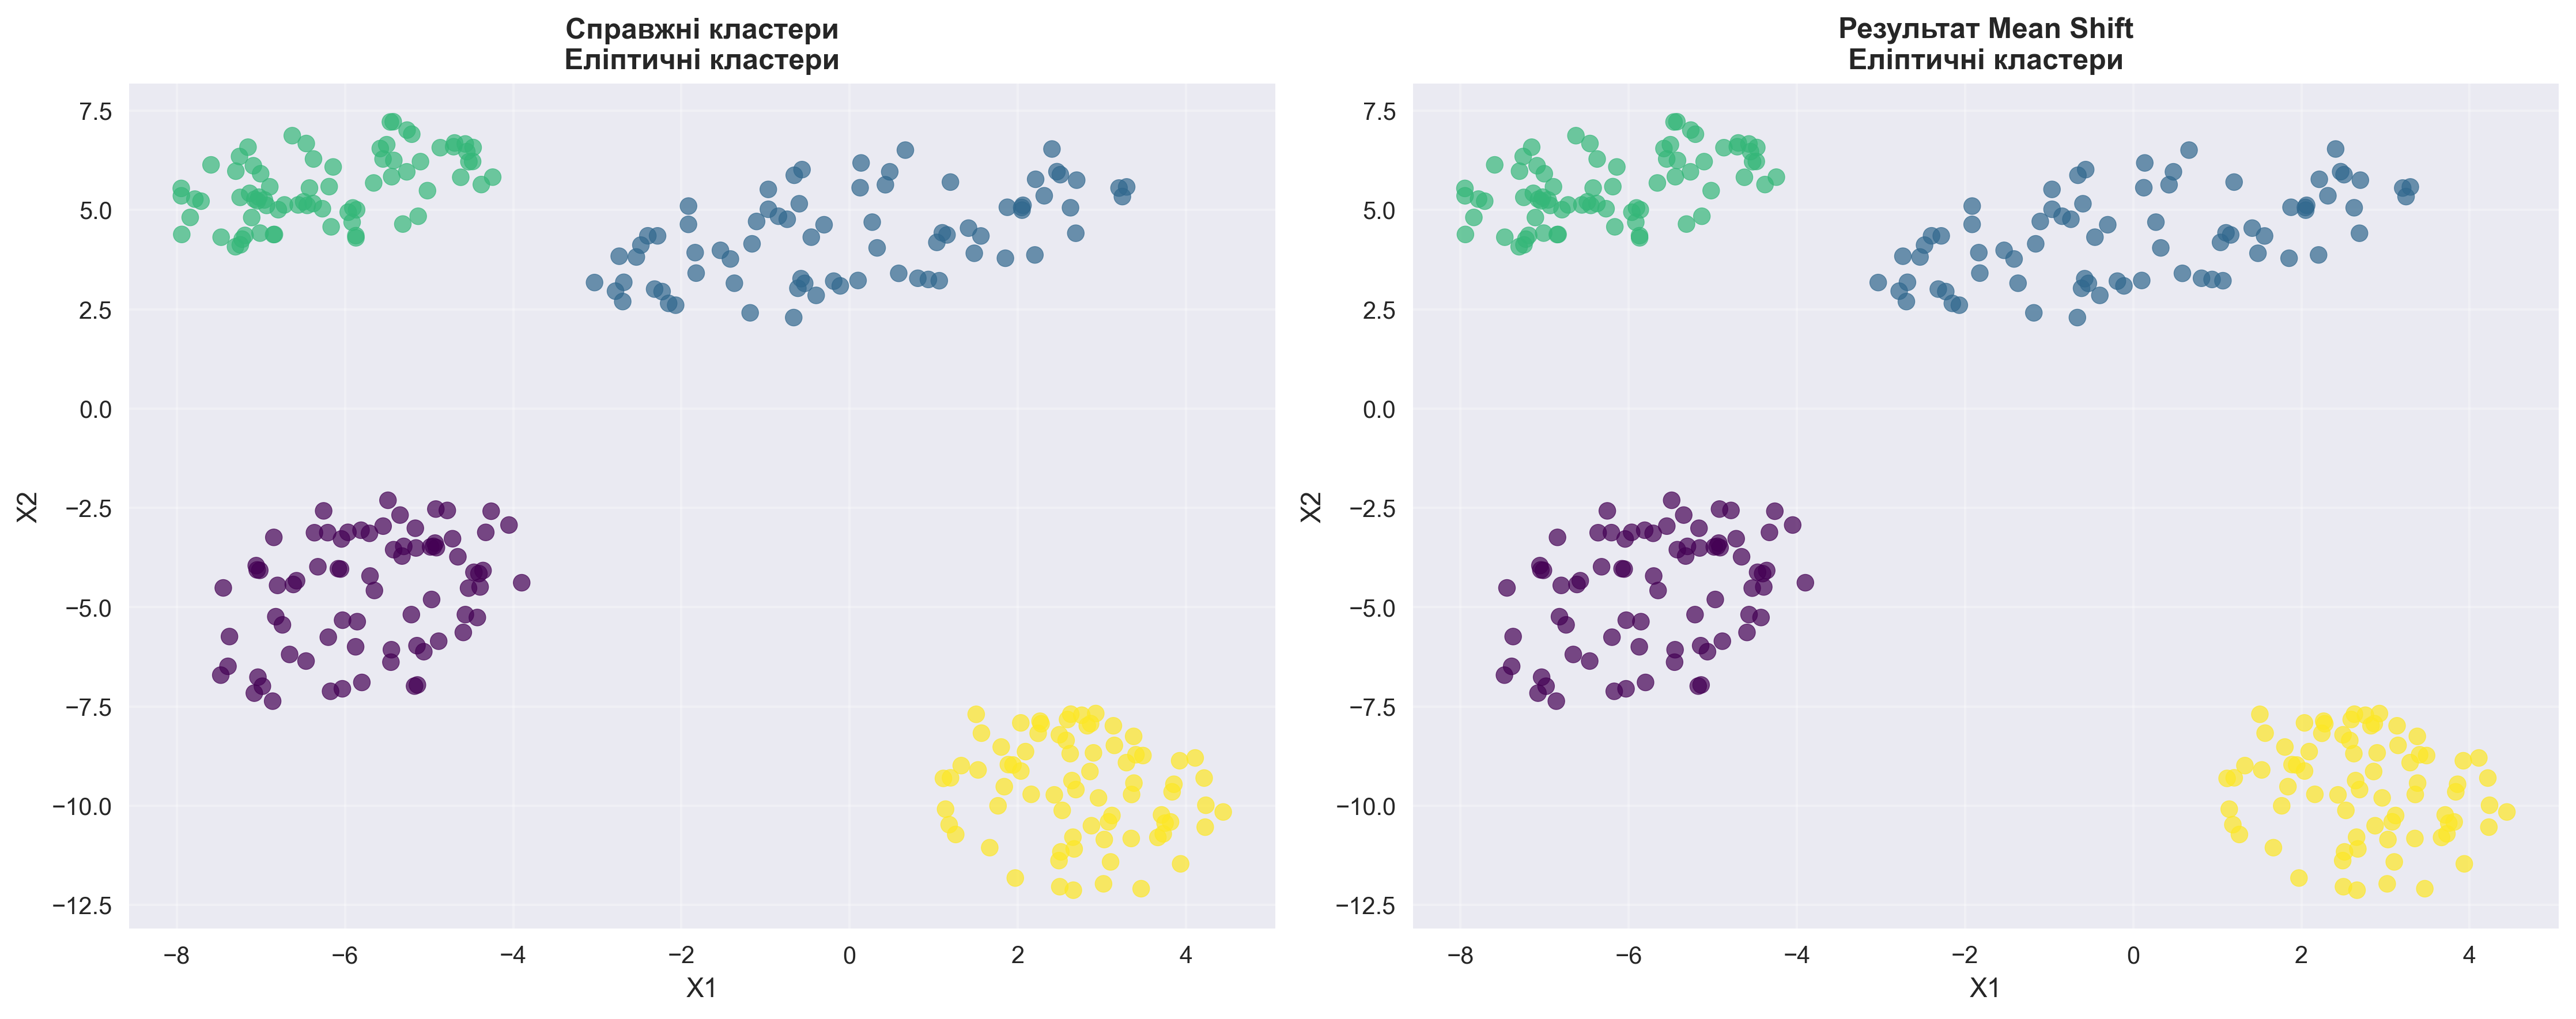
\includegraphics[width=0.8\textwidth]{clustering_visualizations/Mean Shift_Еліптичні_кластери_results.png}
\caption{Результати Mean Shift на еліптичних кластерах}
\label{fig:meanshift_elliptical}
\end{figure}

\subsubsection{Літерні форми}

\begin{figure}[H]
\centering
\includegraphics[width=0.8\textwidth]{clustering_visualizations/K-means_Літерні_форми_results.png}
\caption{Результати K-means на кластерах у формі літер}
\label{fig:kmeans_letters}
\end{figure}

\begin{figure}[H]
\centering
\includegraphics[width=0.8\textwidth]{clustering_visualizations/FOREL_Літерні_форми_results.png}
\caption{Результати FOREL на кластерах у формі літер}
\label{fig:forel_letters}
\end{figure}

\begin{figure}[H]
\centering
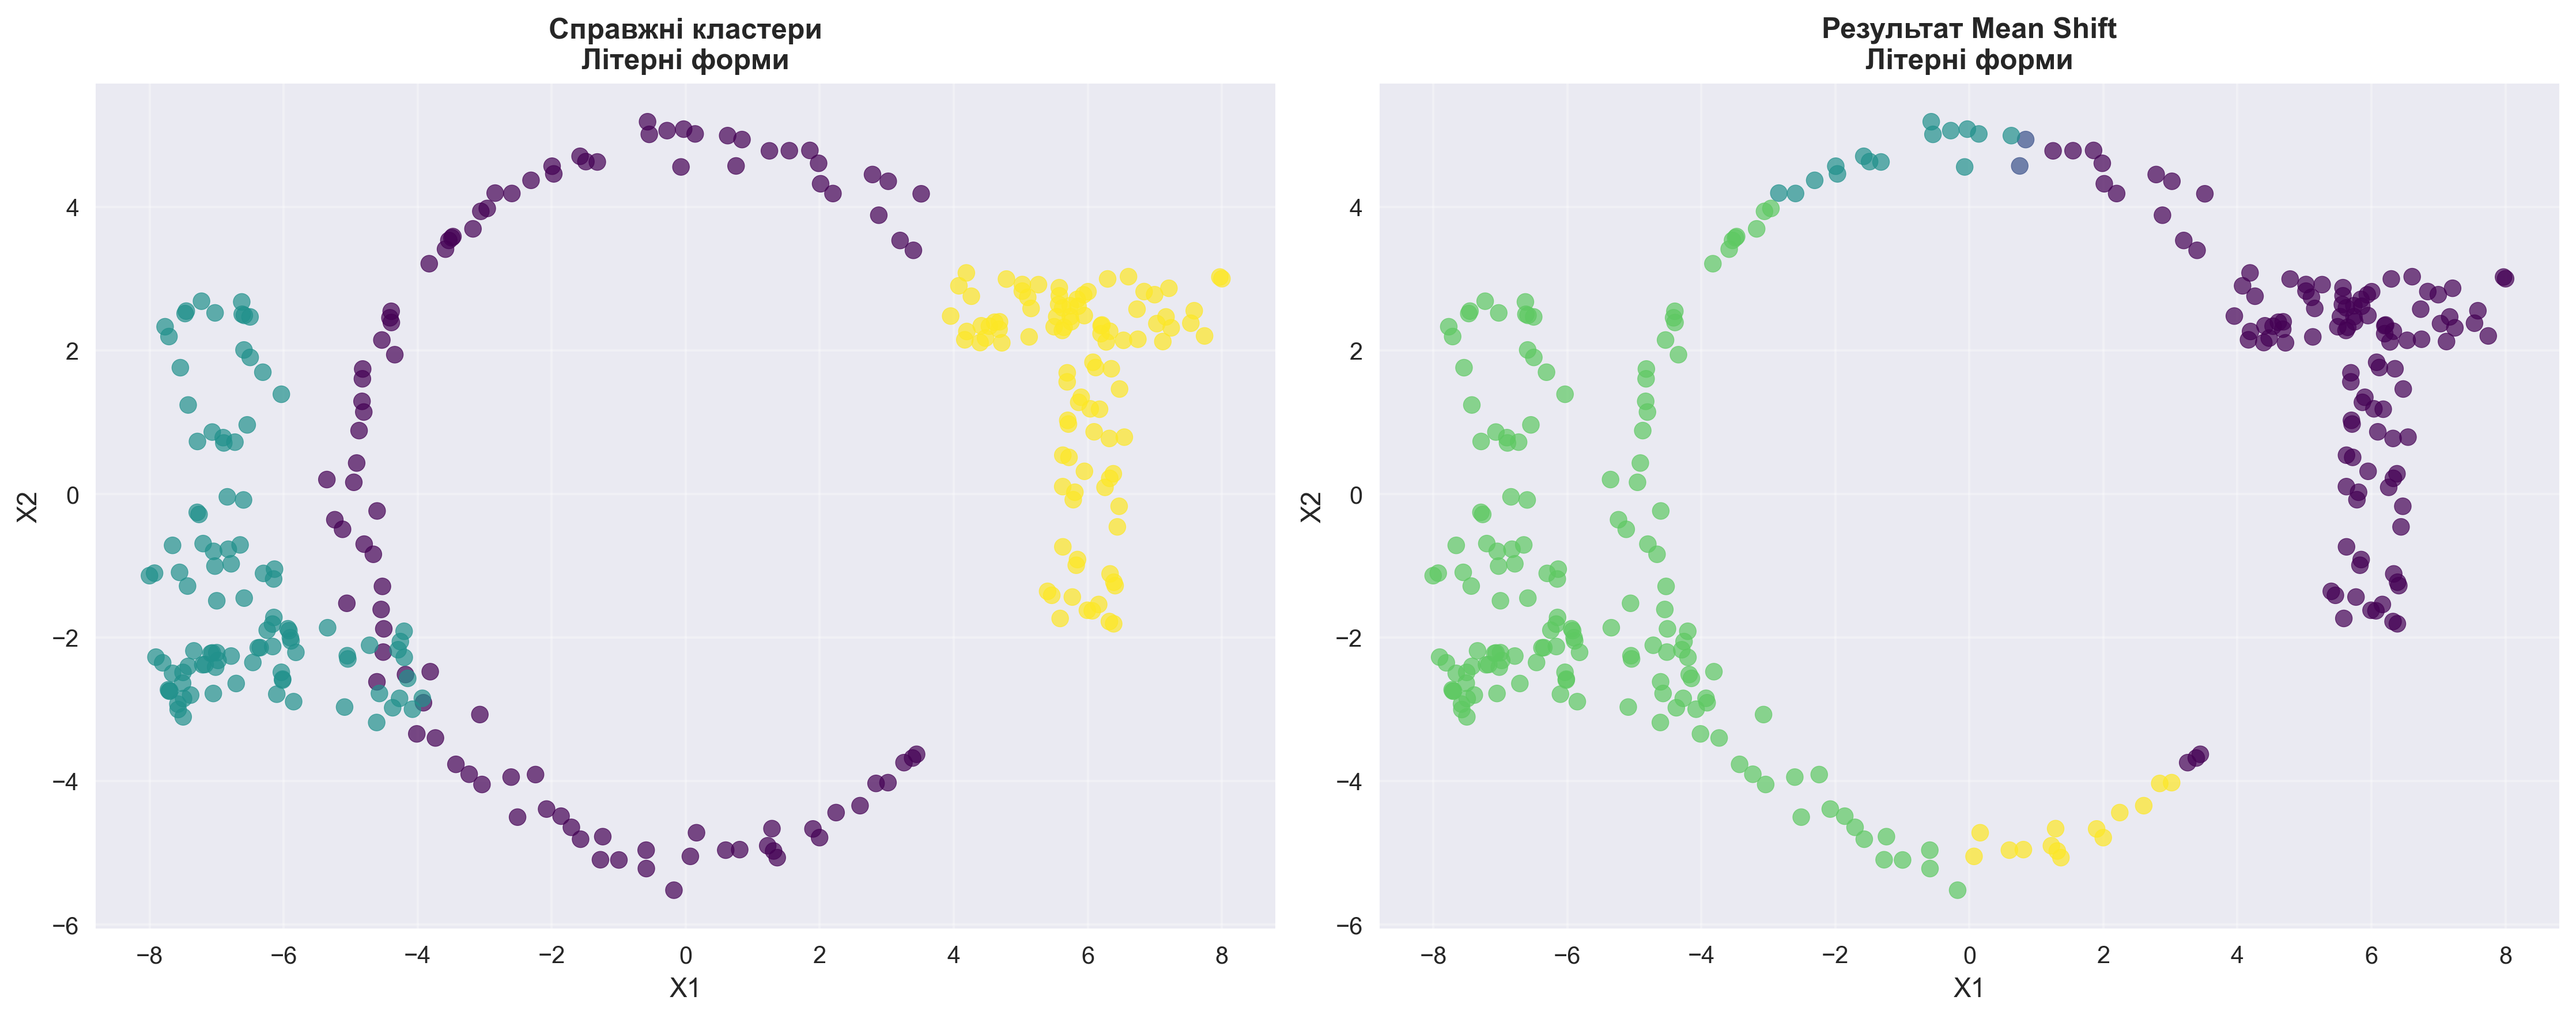
\includegraphics[width=0.8\textwidth]{clustering_visualizations/Mean Shift_Літерні_форми_results.png}
\caption{Результати Mean Shift на кластерах у формі літер}
\label{fig:meanshift_letters}
\end{figure}

\subsubsection{Змішані типи}

\begin{figure}[H]
\centering
\includegraphics[width=0.8\textwidth]{clustering_visualizations/K-means_Змішані_типи_results.png}
\caption{Результати K-means на змішаних типах кластерів}
\label{fig:kmeans_mixed}
\end{figure}

\begin{figure}[H]
\centering
\includegraphics[width=0.8\textwidth]{clustering_visualizations/FOREL_Змішані_типи_results.png}
\caption{Результати FOREL на змішаних типах кластерів}
\label{fig:forel_mixed}
\end{figure}

\begin{figure}[H]
\centering
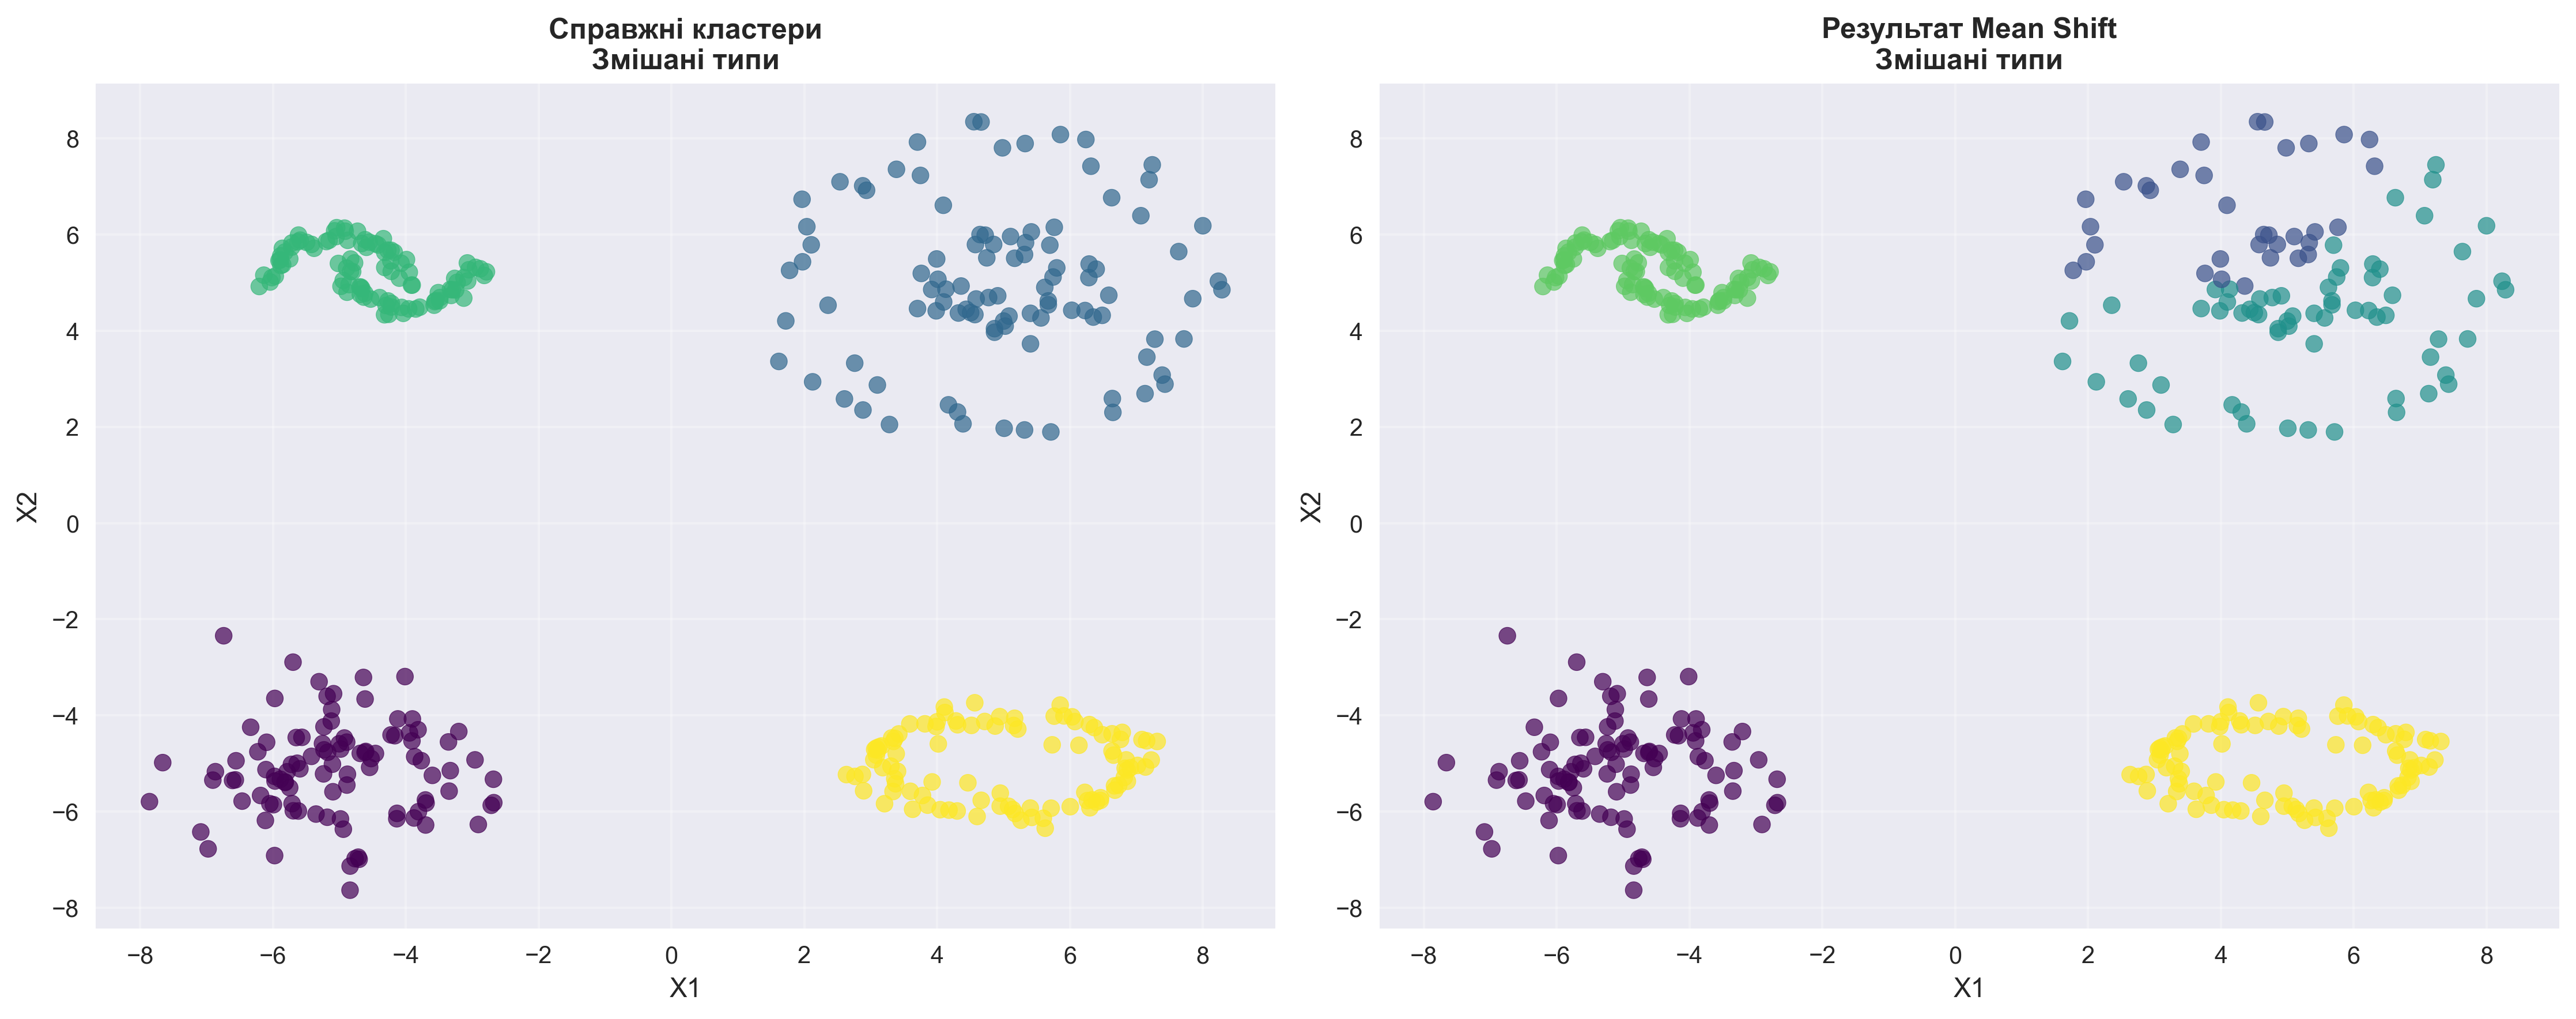
\includegraphics[width=0.8\textwidth]{clustering_visualizations/Mean Shift_Змішані_типи_results.png}
\caption{Результати Mean Shift на змішаних типах кластерів}
\label{fig:meanshift_mixed}
\end{figure}

\subsection{Аналіз стабільності}

\subsubsection{Стабільність K-means}

\begin{figure}[H]
\centering
\includegraphics[width=0.8\textwidth]{clustering_visualizations/K-means_Кругові_кластери_stability.png}
\caption{Аналіз стабільності K-means на кругових кластерах}
\label{fig:kmeans_stability_circular}
\end{figure}

\begin{figure}[H]
\centering
\includegraphics[width=0.8\textwidth]{clustering_visualizations/K-means_Змішані_типи_stability.png}
\caption{Аналіз стабільності K-means на змішаних типах (критична нестабільність)}
\label{fig:kmeans_stability_mixed}
\end{figure}

\subsubsection{Стабільність FOREL}

\begin{figure}[H]
\centering
\includegraphics[width=0.8\textwidth]{clustering_visualizations/FOREL_Кругові_кластери_stability.png}
\caption{Аналіз стабільності FOREL на кругових кластерах}
\label{fig:forel_stability_circular}
\end{figure}

\begin{figure}[H]
\centering
\includegraphics[width=0.8\textwidth]{clustering_visualizations/FOREL_Літерні_форми_stability.png}
\caption{Аналіз стабільності FOREL на літерних формах}
\label{fig:forel_stability_letters}
\end{figure}

\subsubsection{Стабільність Mean Shift}

\begin{figure}[H]
\centering
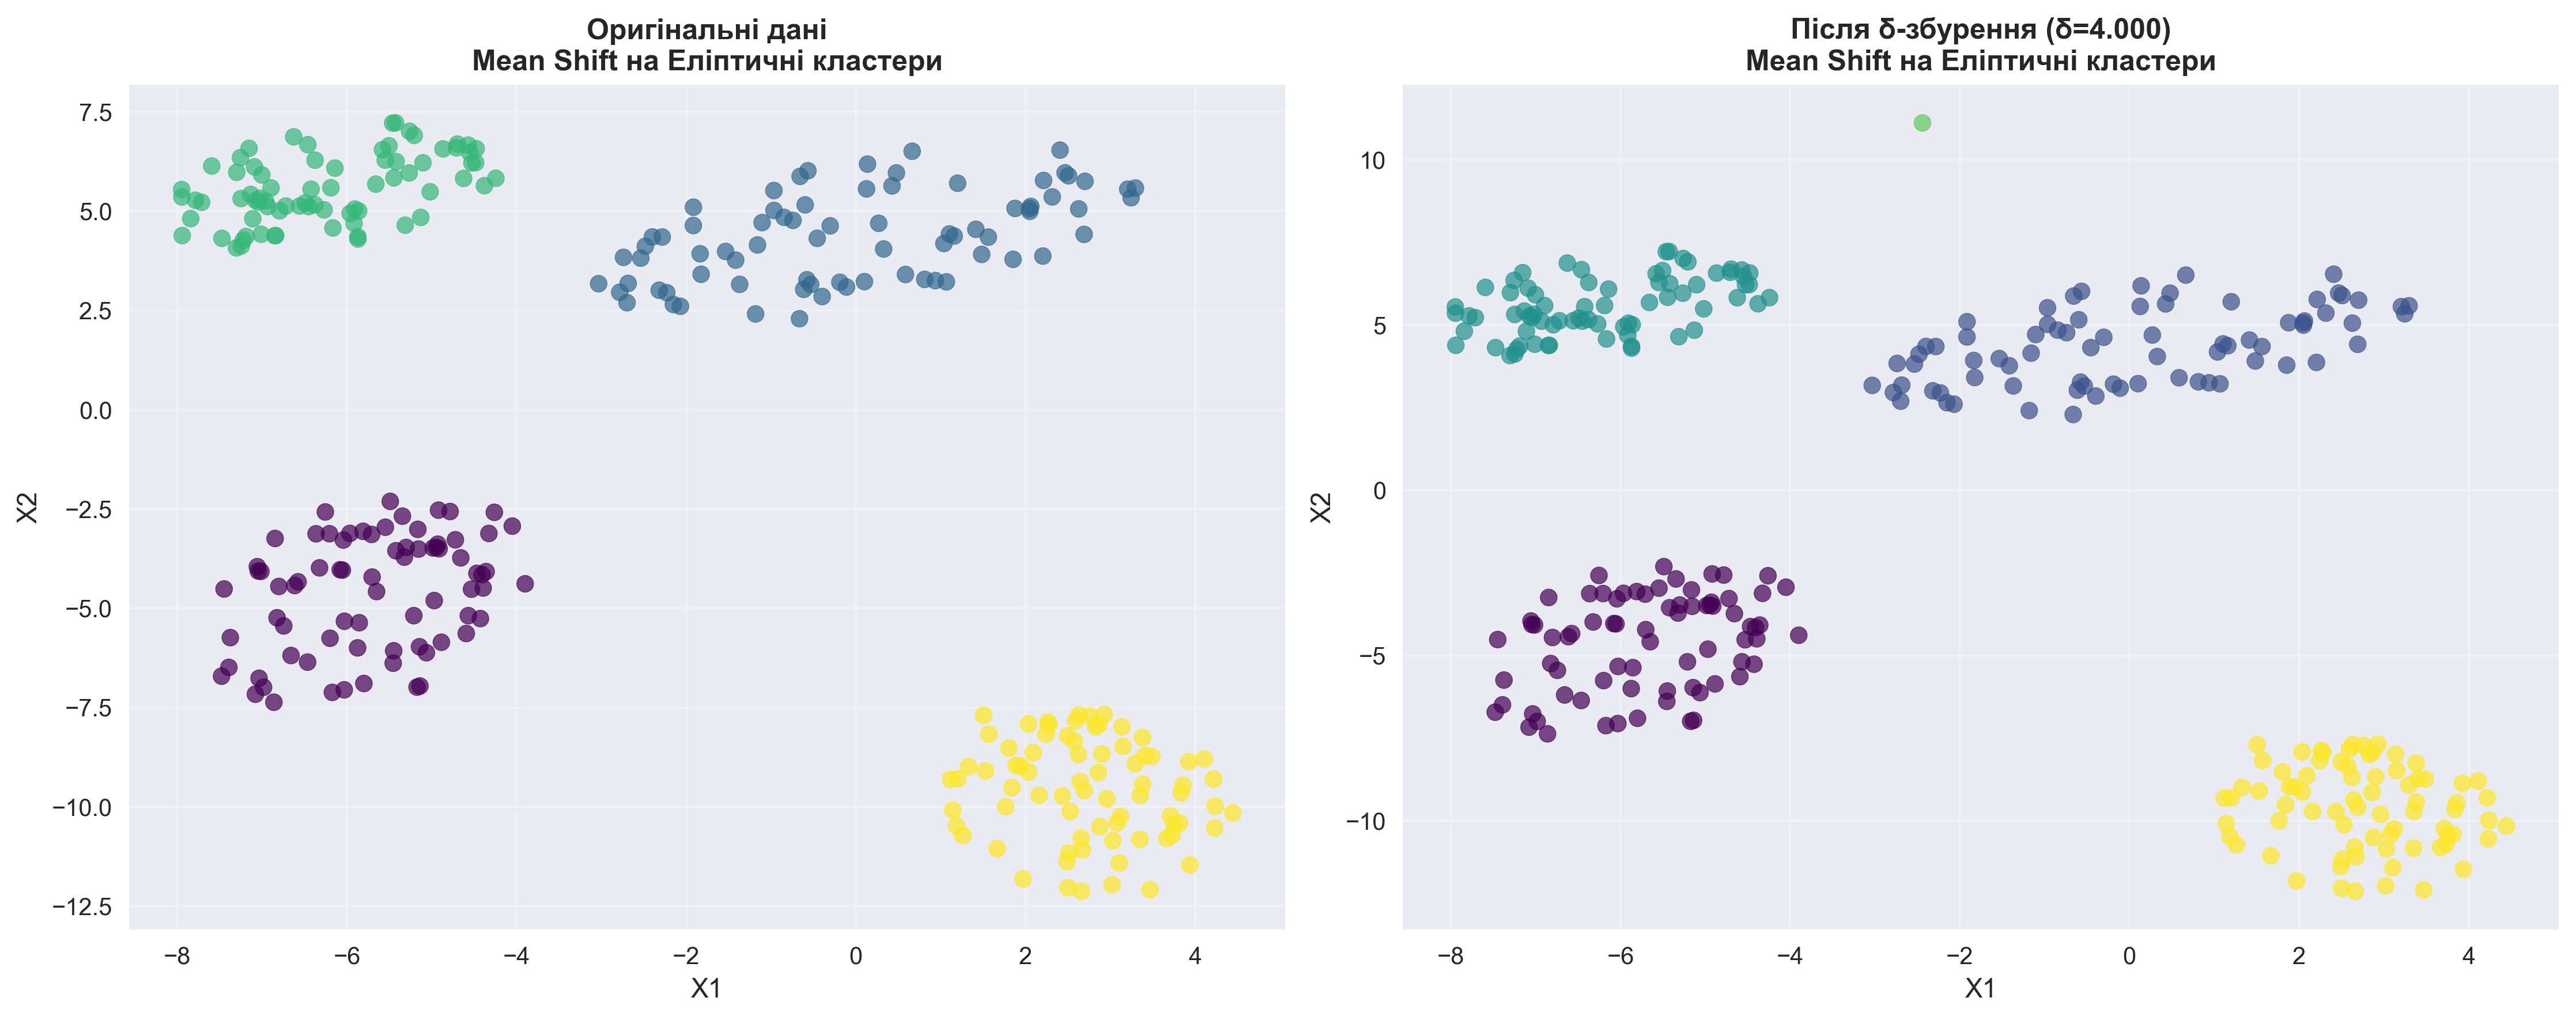
\includegraphics[width=0.8\textwidth]{clustering_visualizations/Mean Shift_Еліптичні_кластери_stability.png}
\caption{Аналіз стабільності Mean Shift на еліптичних кластерах}
\label{fig:meanshift_stability_elliptical}
\end{figure}

\begin{figure}[H]
\centering
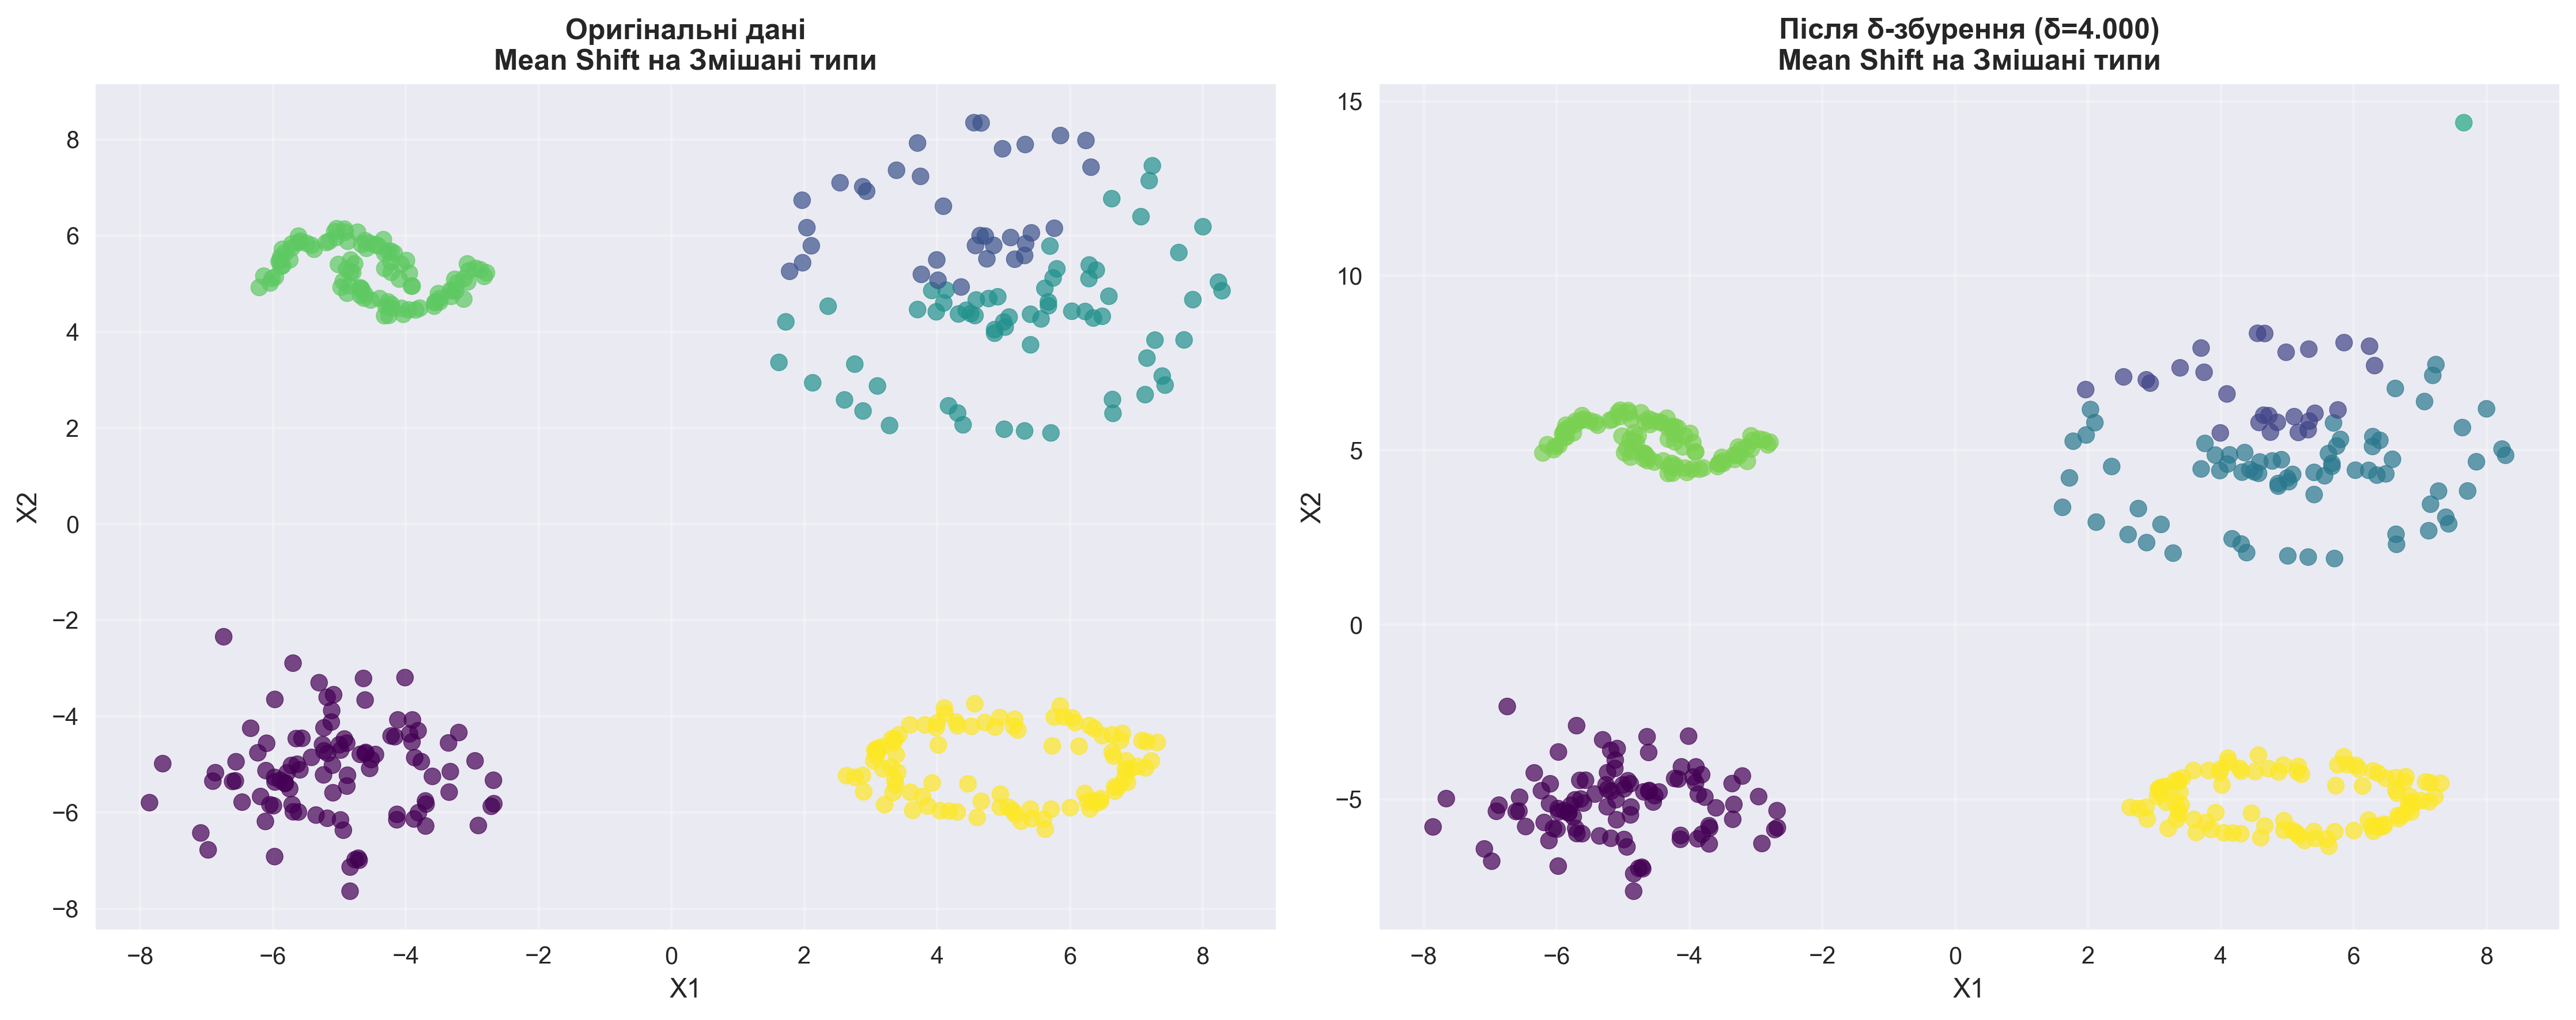
\includegraphics[width=0.8\textwidth]{clustering_visualizations/Mean Shift_Змішані_типи_stability.png}
\caption{Аналіз стабільності Mean Shift на змішаних типах}
\label{fig:meanshift_stability_mixed}
\end{figure}

\subsection{Порівняльні діаграми}

\subsubsection{Продуктивність}

\begin{figure}[H]
\centering
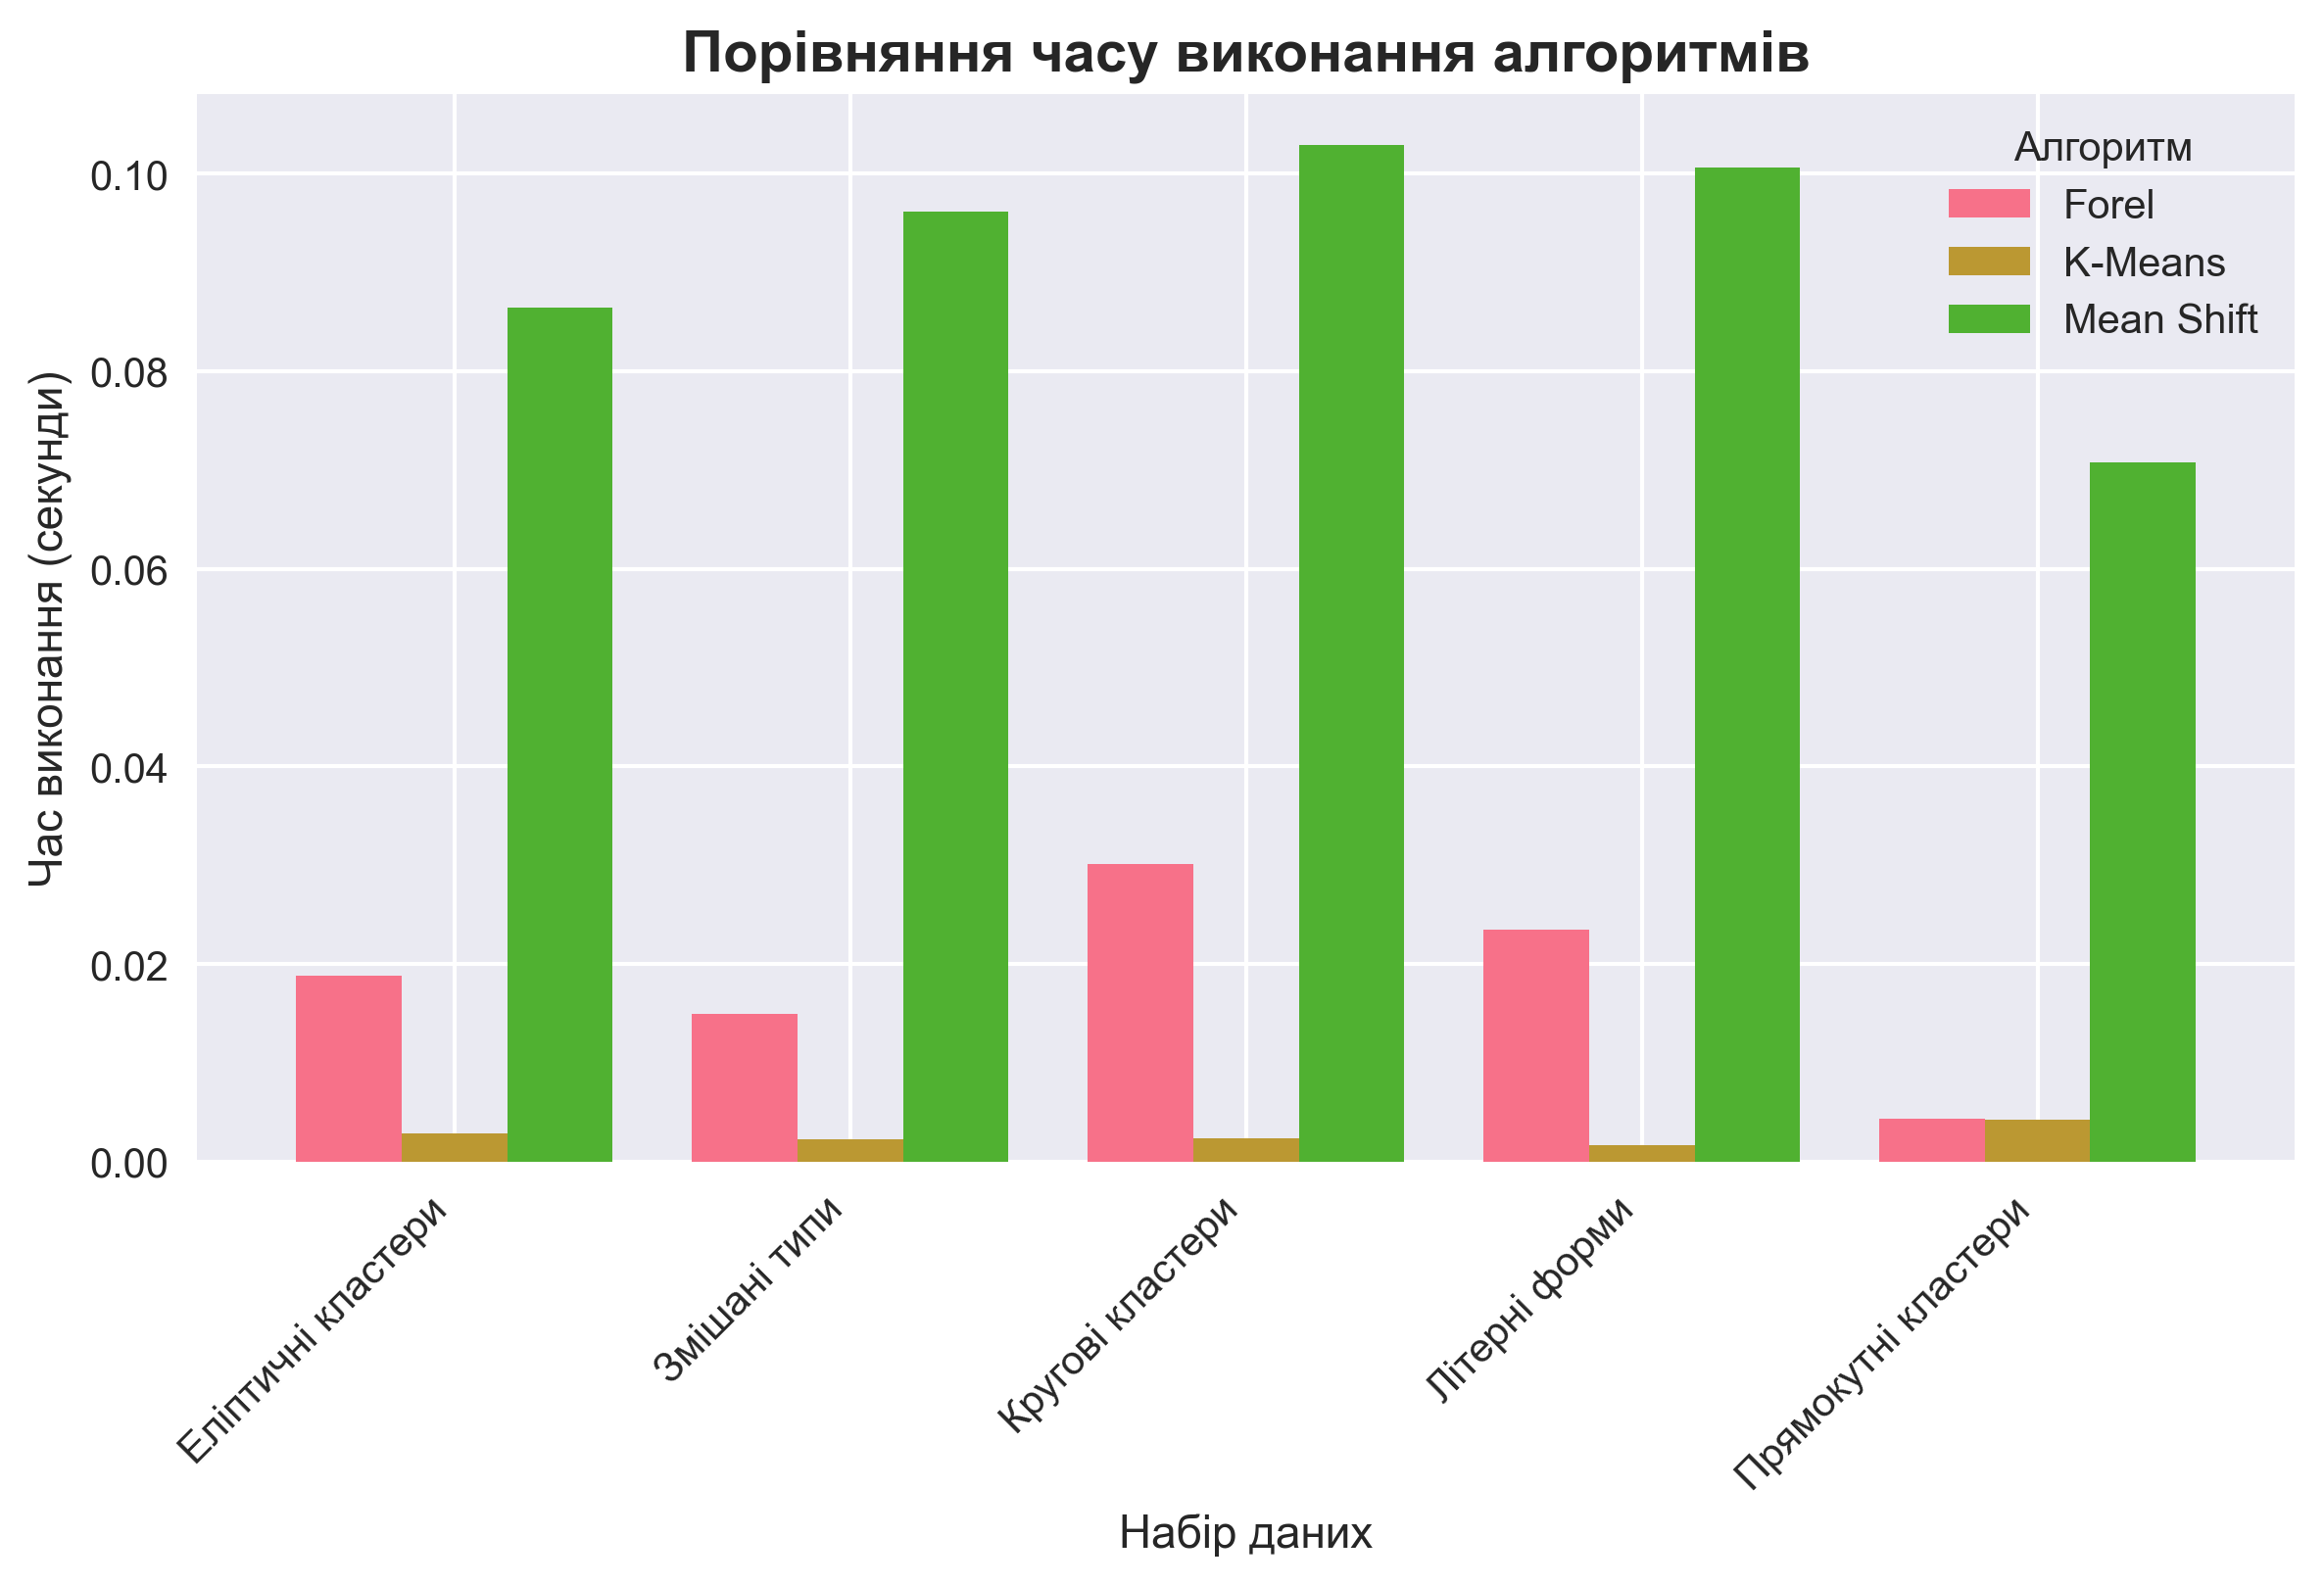
\includegraphics[width=0.9\textwidth]{clustering_visualizations/execution_time_comparison.png}
\caption{Порівняння часу виконання алгоритмів на різних типах даних}
\label{fig:time_comparison}
\end{figure}

\begin{figure}[H]
\centering
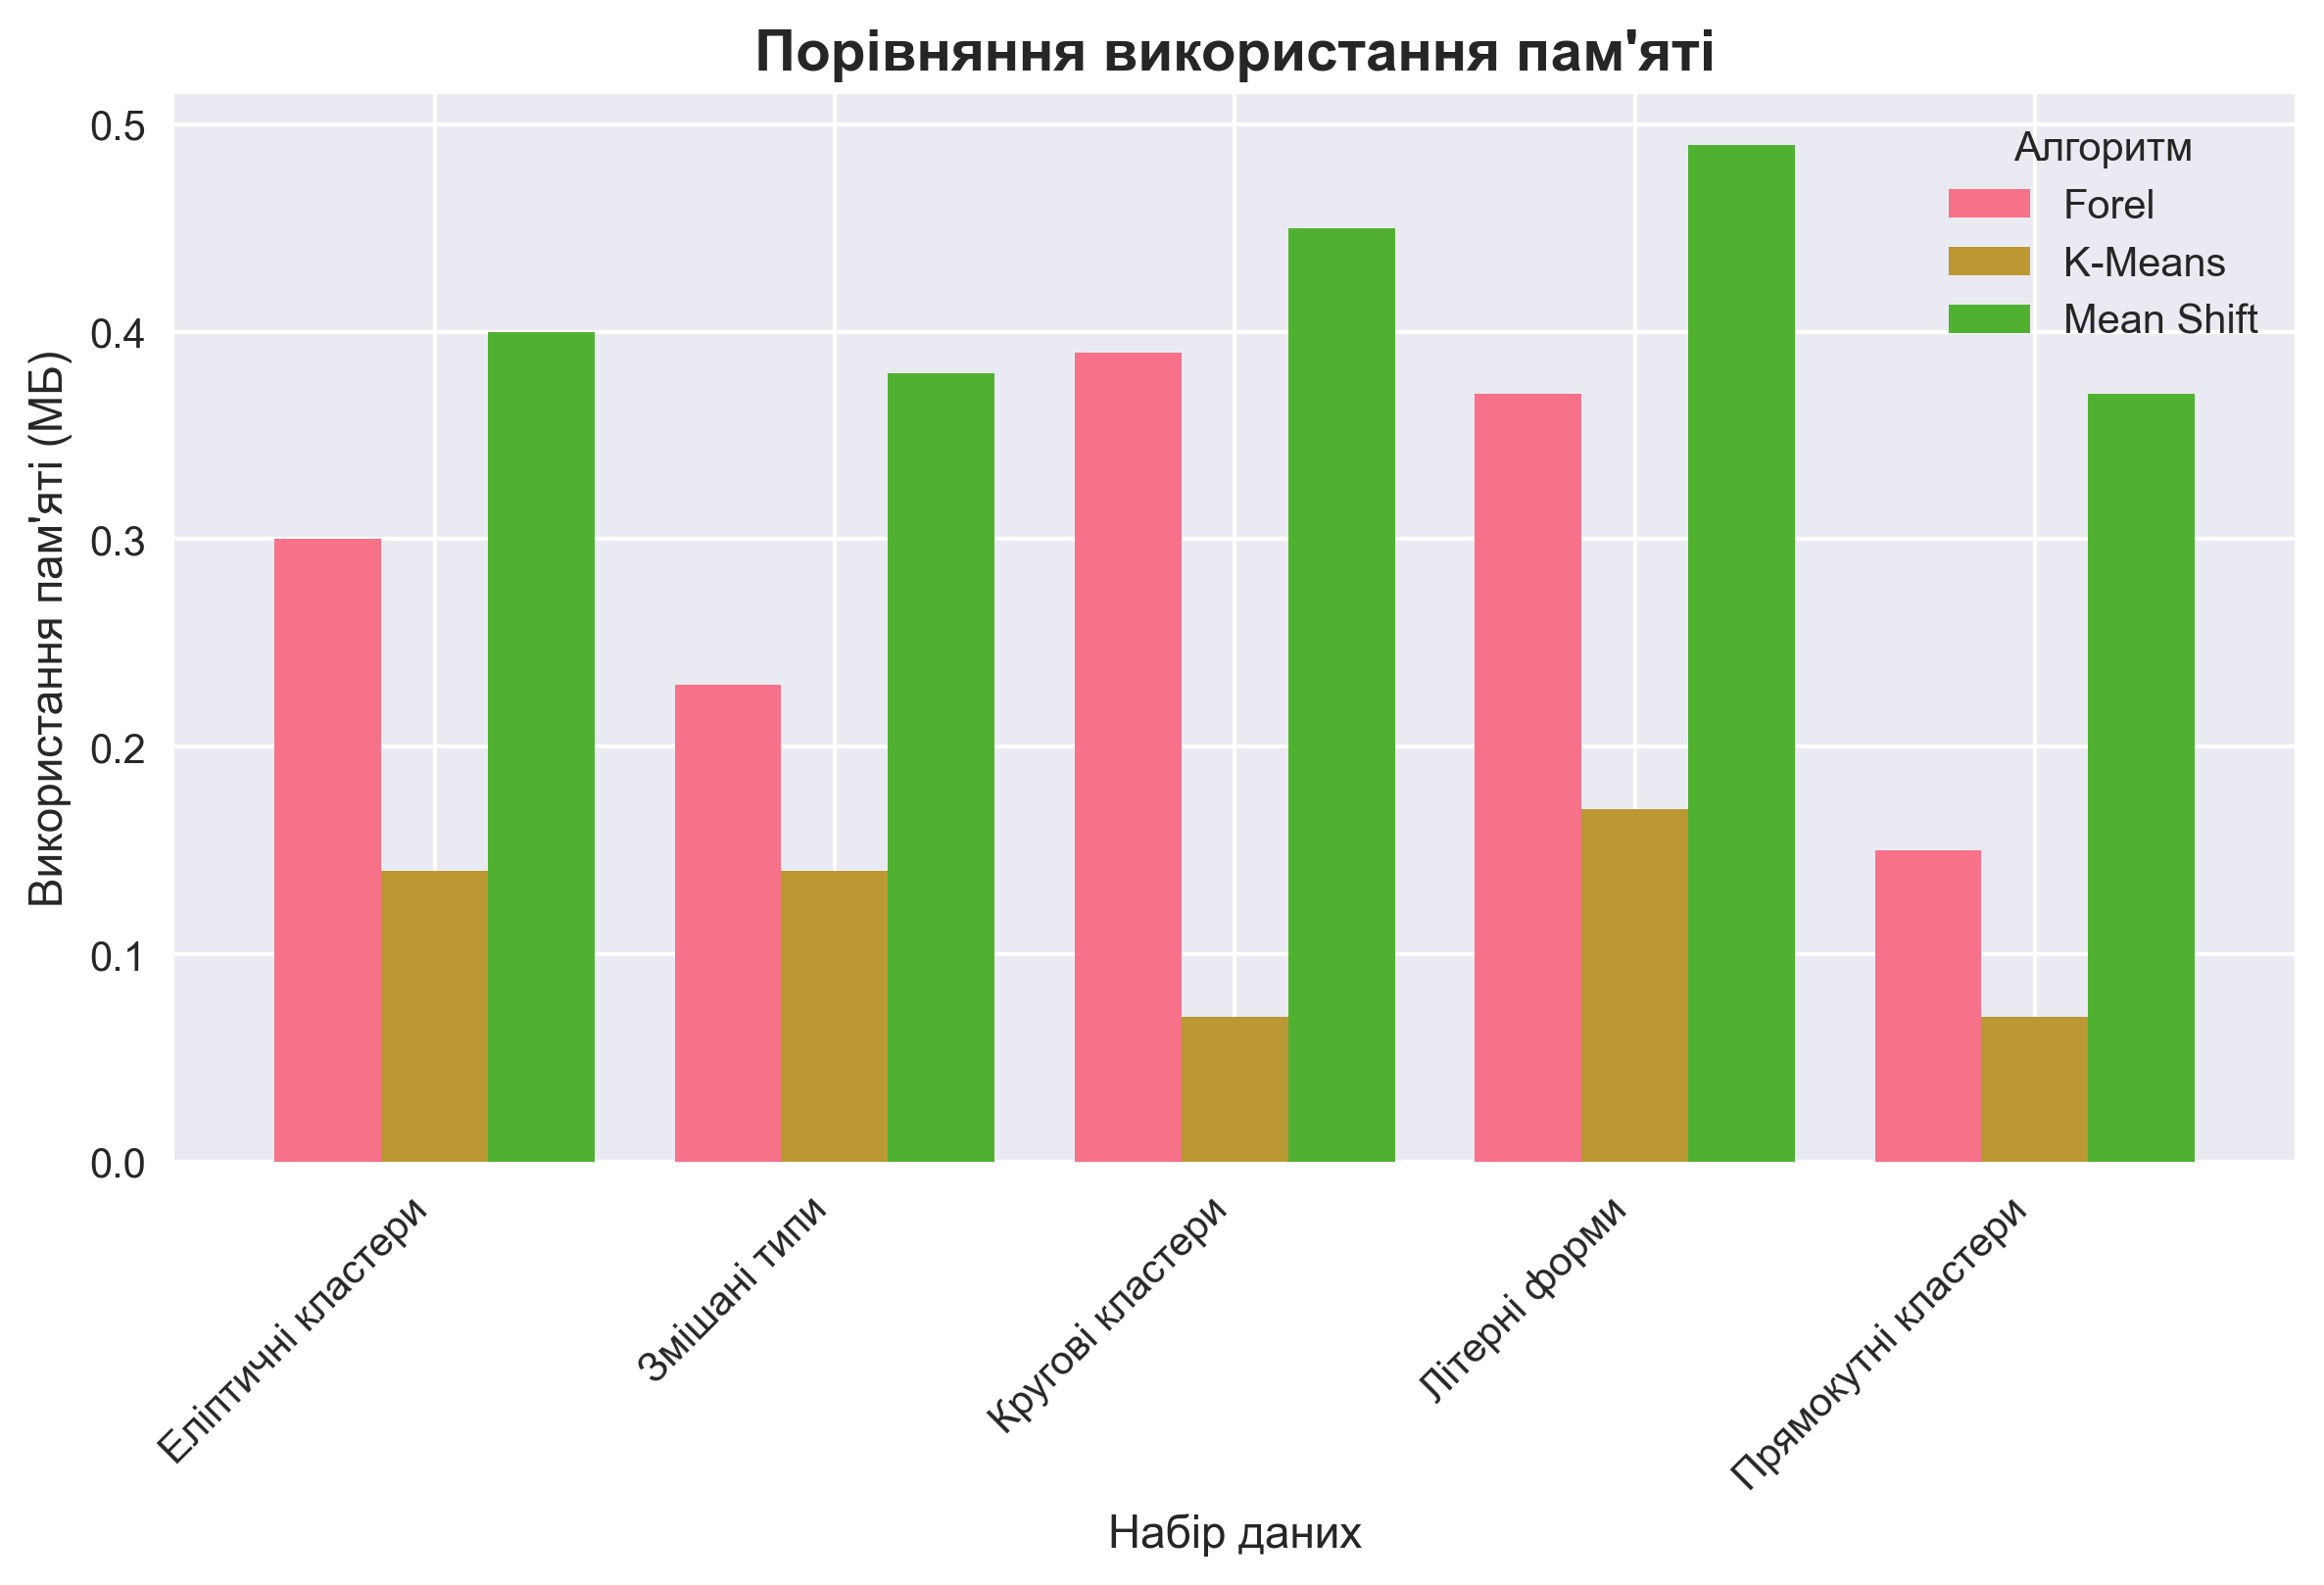
\includegraphics[width=0.9\textwidth]{clustering_visualizations/memory_usage_comparison.png}
\caption{Порівняння використання пам'яті алгоритмами}
\label{fig:memory_comparison}
\end{figure}

\end{document}